\documentclass{report}
\usepackage[T1]{fontenc} % Fontes T1
\usepackage[utf8]{inputenc} % Input UTF8
\usepackage[backend=biber, style=ieee]{biblatex} % para usar bibliografia
\usepackage{csquotes}
\usepackage[portuguese]{babel} %Usar língua portuguesa
\usepackage{blindtext} % Gerar texto automaticamente
\usepackage[printonlyused]{acronym}
\usepackage{hyperref} % para autoref
\usepackage{graphicx}
\usepackage{indentfirst}
\usepackage{listings}
\usepackage{xcolor}


\definecolor{codegreen}{rgb}{0,0.6,0}
\definecolor{codegray}{rgb}{0.5,0.5,0.5}
\definecolor{codepurple}{rgb}{0.58,0,0.82}
\definecolor{backcolour}{rgb}{0.95,0.95,0.92}

\lstdefinestyle{mystyle}{
  backgroundcolor=\color{backcolour},   commentstyle=\color{codegreen},
  keywordstyle=\color{magenta},
  numberstyle=\tiny\color{codegray},
  stringstyle=\color{codepurple},
  basicstyle=\ttfamily\footnotesize,
  breakatwhitespace=false,         
  breaklines=true,                 
  captionpos=b,                    
  keepspaces=true,                 
  numbers=left,                    
  numbersep=5pt,                  
  showspaces=false,                
  showstringspaces=false,
  showtabs=false,                  
  tabsize=2
}


\lstset{style=mystyle}


\bibliography{bibliografia}


\begin{document}
%%
% Definições
%
\def\titulo{Servidor WEB com Persistência}
\def\data{DATA}
\def\autores{João Alcatrão \
José Jordão \ Mónica Pereira \ Pedro Costa}
\def\autorescontactos{(76763) jalcatrao@ua.pt \\
(103075) josemmjordao@ua.pt \\ 
(102735) monica.alex.pereira12@ua.pt \\
(112682) pedromsc37@ua.pt}
\def\versao{VERSAO FINAL}
\def\departamento{Dept. de Eletrónica, Telecomunicações e Informática}
\def\empresa{Universidade de Aveiro}
\def\logotipo{ua.pdf}
%
%%%%%% CAPA %%%%%%
%
\begin{titlepage}

\begin{center}
%
\vspace*{50mm}
%
{\Huge \titulo}\\ 
%
\vspace{10mm}
%
{\Large \empresa}\\
%
\vspace{10mm}
%
{\LARGE \autores}\\ 
%
\vspace{30mm}
%
\begin{figure}[h]
\center
\includegraphics{\logotipo}
\end{figure}
%
\vspace{30mm}
\end{center}
%
\begin{flushright}
\versao
\end{flushright}
\end{titlepage}

%%  Página de Título %%
\title{%
{\Huge\textbf{\titulo}}\\
{\Large \departamento\\ \empresa}
}
%
\author{%
    \autores \\
    \autorescontactos
}
%
\date{\today}
%
\maketitle

\pagenumbering{roman}

%%%%%% RESUMO %%%%%%
\begin{abstract}
Neste relatório encontra-se uma demonstração e explanação, em texto e imagem, da aplicação WEB realizada e baseada no Tutorial 2 – Servidor WEB com Persistência, e complementada com funcionalidades de registo/login e manipulação de imagens.

\linebreak
\bigskip

 	A nossa aplicação é composta por uma interface (que é em si composta por elementos html, css e javascript) que pode ser utilizada através do browser, uma base de dados (com uso de sql) para efeitos de persistência, e o servidor WEB em si (programada em python).

\linebreak
\bigskip
  
	A interface é utilizada para interagir de maneira simples e elegante com o servidor WEB, através de requests /GET e /POST. O servidor, em prol dos pedidos que recebe da interface, pode atualizar a base de dados, de modo a guardar dados que se desejem guardar, mesmo caso o servidor seja desligado.

\linebreak
\bigskip

	A aplicação WEB serve sobretudo para carregar, guardar e visualizar imagens e manipulá-las, permitindo também que sejam feitos comentários e “likes” (e “dislikes”) nessas imagens. Para utilizar estas funcionalidades, é preciso que haja um registo, e um posterior login por parte de quem deseja usufruir delas.

\linebreak
\bigskip
 
	Todas as funcionalidades apresentadas funcionam como pretendemos que funcionem, e todos os objetivos que foram propostos para a realização deste projeto foram alcançados, e ao longo do relatório, iremos demonstrar exemplos que o demonstrem, acompanhados de imagens, tanto do resultado, como do código que o produz, bem como de explicações que visam clarificar como foram implementados.

\end{abstract}




\tableofcontents
% \listoftables     % descomentar se necessário
% \listoffigures    % descomentar se necessário


%%%%%%%%%%%%%%%%%%%%%%%%%%%%%%%
\clearpage
\pagenumbering{arabic}

%%%%%%%%%%%%%%%%%%%%%%%%%%%%%%%%
\chapter{Introdução}
\label{chap.introducao}

\subsection{Tema}

O projeto que nos foi proposto fazer tem como objetivo principal o desenvolvimento de uma aplicação WEB que permita gerir imagens, através do carregamento, visualização, manipulação, e até comentário e apreciação (através de gostos/desgostos) das mesmas.

\linebreak
\bigskip

Mais especificamente, a aplicação deve permitir ao utilizador: carregar imagens à sua escolha com identificação do autor, de um nome que a identifique a imagem, e a data e hora de carregamento da mesma; visualizar as imagens existentes, todas ou filtradas por um autor em particular; visualizar uma imagem em particular, com todos os comentários e votos feitos pelos utilizadores; e acrescentar comentários a imagens. Também deve ter um sistema de pontuação de popularidade de uma imagem através de um sistema de votação de gostos/desgostos (likes/deslikes). A aplicação deve também permitir a manipulação de imagens através de algoritmos implementados para esse efeito. Finalmente, a aplicação, no nosso caso, também faz uso de um sistema de registo/login.

\subsection{Motivação}

Nós começámos este projeto ainda antes de ele nos ter sido proposto, visto que ele baseia-se extensamente no Tutorial 2 – Servidor WEB com Persistência; um tutorial que se encontra para fazer (e que fizemos atempadamente) na parte 2 do Guião 6 da disciplina. Este guião é extensivo e complexo – é preciso ter conhecimento em python, html, css, javascript, e sql para o realizar. Este mesmo conhecimento é assim requerido para realizar a aplicação WEB proposta, que implica também a aplicação de matéria dada e conhecimento obtido em vários outros módulos da disciplina; módulos que se fundamentam na aprendizagem e no uso de matérias acerca de, por exemplo, bases de dados relacionais, da Framework Cherrypy, de criptografia, de testes, e de algoritmos de manipulação de imagem.

\subsection{Estrutura}

\subsubsection{Organização estrutural}

A nossa solução é composta por 3 componentes inter-dependentes para assegurar o correto desenvolvimento e o bom funcionamento da aplicação proposta. Estes componentes são: a interface (que contém páginas html, css, e scripts javascript, que permitem ao utilizador interagir com as mesmas, que se encarregam de transmitir os dados recebidos para o servidor WEB para que se possa obter os resultados desejados), o servidor WEB em si (que consiste num conjunto de métodos e classes em python, que conseguem receber os dados da interface através da dinâmica entre os requests recebidos da mesma e da Framework cherrypy, e que permite fazer pesquisas e alterações na base de dados, conforme seja pedido, e que ainda permite guardar imagens em pastas do sistema de ficheiros, conforme seja necessário [tmp] ou desejado [uploads]), e a base de dados (relacional, em sql, que confere persistência à aplicação em função dos comandos que o servidor executa sobre ela).

\linebreak
\bigskip
    
	Estas 3 componentes encontram-se organizadas no sistema de ficheiros do sistema operativo (juntamente com pastas auxiliares tmp e uploads) da seguinte forma:

\begin{figure}[!hbtp]
        \centering 
        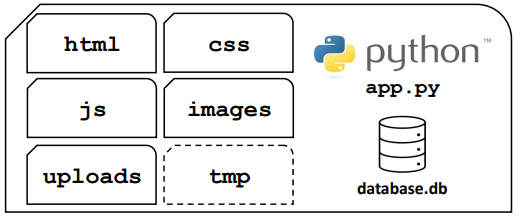
\includegraphics[scale=0.550]{Images/estrutura.png}
        \caption{\label{Estrutura}Organização dos elementos que constituem a aplicação WEB}
    \end{figure}

\newpage
\subsubsection{Organização visual}


Visto que a interface é o único meio por onde o utilizador pode comunicar com a aplicação por um todo, é importante também definir bem como é que o utilizador pode prosseguir de modo a conseguir obter o que deseja da aplicação.
\linebreak
  
	Tendo em conta o tema e propósito da aplicação de gerir imagens, através do carregamento, visualização, manipulação, e apreciação das mesmas, definimos, na interface, que consiste em páginas html, css, e scripts javascript, e que é acessível através do browser, as seguintes páginas, acessíveis a partir da barra de navegação da página de início da interface:
-página de início (Home), cujo propósito é situar o utilizador numa posição confortável, com apenas a informação essencial visível (como o tema da aplicação, e os nomes das páginas que correspondem às funcionalidades de que o utilizador pretenda usufruir);

\begin{enumerate}
    \item \textbf{Gallery Page}
    - cuja função é listar todas as imagens presentes no sistema, ordenadas por ordem ascendente do nome, permitindo a sua visualização. As imagens em si estarão armazenadas no sistema de ficheiros da aplicação Web. As imagens apresentam o nome dado pelo autor que as carregou, mas no sistema de ficheiros, cada imagem é identificada por um nome criado a partir da síntese do conteúdo da própria imagem. Esta página apresenta assim uma lista de imagens e permite que elas possam ser filtradas pelo nome do autor (total ou parcial).
    
\linebreak

 Quando uma destas imagens é selecionada, é aberta uma nova página autónoma (Image) que apresenta todas as suas propriedades (autor, nome, hora e data de upload no sistema e comentários efetuados pelos utilizadores). Esta página permite que o utilizador acrescente um novo comentário à imagem selecionada, e também apresenta um sistema de apreciação/pontuação de popularidade da imagem (likes/deslikes).

 \linebreak
\bigskip

    \item \textbf{Upload Page}
    - página de carregamento de imagens, que permite o carregamento de uma nova imagem no sistema. Cada imagem tem associado um nome e o utilizador que a carregou no sistema, bem como a data e hora de carregamento.

    \newpage

    \item \textbf{Image Manipulation Page}
    - página de manipulação de imagens , que permite ao utilizador escolher um método/algoritmo de processamento de imagens, e selecionar a imagem (ou imagens, dependendo do método de manipulação que escolher) que pretende alterar.
\linebreak
  
     É de notar que o utilizador não precisa de carregar as imagens que pretende alterar anteriormente a partir da página de Upload, visto que poderá só querer carregar uma imagem que tenha manipulado a seu gosto, e não carregar a original, e a manipulada (pelo que não tem que escolher uma imagem previamente carregada e guardada no servidor, mas sim uma no seu computador pessoal). No caso de manipulações que requerem múltiplas imagens, também seria pouco agradável ter que carregar todas essas imagens primeiro no servidor antes de as poder manipular, o que poderia causar maior frustração caso o utilizador afinal não gostasse do resultado da manipulação.
\linebreak
   
     Além das imagens, o utilizador pode ainda escolher um conjunto de opções ou inserir algum input para personalizar mais ao seu gosto a imagem manipulada, dependendo do método de manipulação alterada. Manipulação de imagens é algo complexo, com resultados por vezes imprevisíveis e surpreendentes, pelo que nesta página, o utilizador tem muitas mais opções a considerar comparativamente às outras páginas, para que tenha maior controlo sobre o que realmente deseja fazer com as suas imagens.

    \item \textbf{About Page}
    - página About, que contém informações sobre nós, os realizadores, da aplicação. 
\end{enumerate}

\newpage


\begin{figure}[!hbtp]
        \centering 
        
\includegraphics[scale=0.40]{Images/organização interface.png}
        \caption{\label{Estrutura}Barra de navegação da página de início}
    \end{figure}

É de salientar um ponto importante: esta barra de navegação útil e todas estas funcionalidades de que se pode usufruir a partir da página de início, só são disponibilizadas após haver um login efetuado com sucesso.

\linebreak
\bigskip

Existe assim, uma outra página, que controla o acesso a todas as outras (exceto a About, que tem acesso livre), que é a página de login/registo. A função desta página é permitir aos utilizadores registarem-se e fazerem login, o que os distinguirá dos outros utilizadores.
	Para não frustrar o utilizador, a efetuação de registo/login é bastante direta, requerendo apenas um nome de utilizador e uma password, e quando um utilizador fizer login e aceder às páginas de Upload, ou clicar numa imagem na Galeria para comentar, verá que o campo de autor já estará preenchido com o seu nome de utilizador – assim, ninguém poderá comentar ou carregar imagens com o nome particular de um utilizador, a não ser o próprio.   





\chapter{Metodologia}
\label{chap.metodologia}

Nesta secção iremos demonstrar como implementámos as diferentes componentes da nossa solução, e explicar como funciona ao certo cada funcionalidade, com exemplos de código para sustentar a explicação.

\linebreak
\bigskip

	A estrutura desta secção segue um modelo de ligação entre as diversas componentes que no seu todo constituem uma funcionalidade no seu todo (por exemplo, é indicada uma funcionalidade – digamos, o carregamento de imagens – e explicamos como implementámos esta funcionalidade (começando pela tabela respetiva na base de dados, seguido da criação de elementos html e funções em javascript para obter da interface os dados necessários da imagem em si, e finalmente, no servidor, explicitamos como é que os dados obtidos da interface são manipulados de modo a guardar a imagem no sistema de ficheiros do servidor e a adicionar uma entrada com a informação de nome, autor, data na base de dados, onde se começou).


\section{Base de Dados}

\paragraph{}
    Começando pela componente mais simples de implementar e de descrever, a nossa base de dados relacional permite registar diversos dados e informações imprescindíveis ao bom funcionamento da nossa solução, como o registo dos utilizadores e das suas respetivas passwords.

	A base de dados é composta por 4 tabelas; uma para guardar informações dos utilizadores (accounts), outra para guardar informações das imagens (images), outra para guardar informações dos comentários (comments), e outra para guardar informações dos likes/dislikes (votes).

 \newpage
    A sua implementação mostra-se de seguida.



\begin{figure}[!hbtp]
        \centering 
        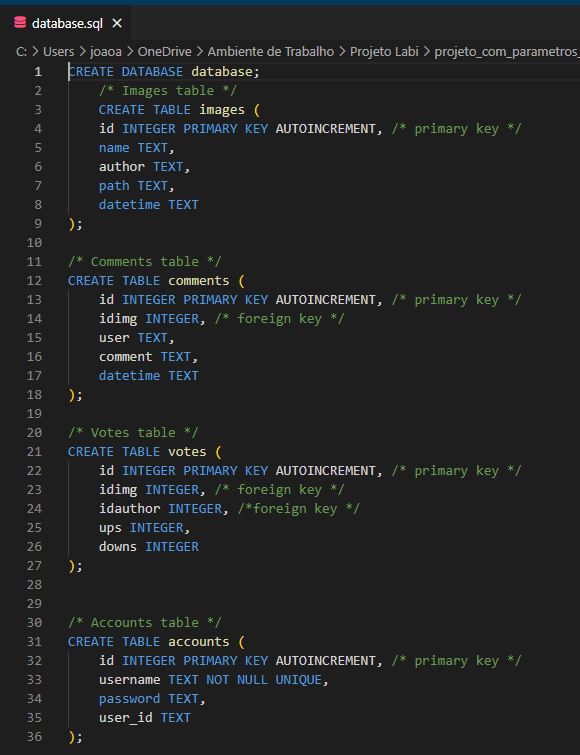
\includegraphics[scale=0.7]{Images_code/3 - base de dados.png}
        \caption{\label{Metodologia}Código de implementação da base de dados.}
\end{figure}

Analisemos agora com mais detalha como cada tabela interage com a aplicação, seguindo o modelo descrito acima.    
\newpage

\subsection{Tabela accounts – o que é e como interagir com ela}

A tabela accounts contém 4 campos: um id inteiro auto-incrementado, um campo de texto único para os nomes de utilizadores (username), um campo de texto para as passwords (password), e um campo de texto denominado user\_id, que é um parâmetro essencial para garantir que utilizadores diferentes possam aceder à interface em simultâneo e, ao mesmo tempo, garantir a sua individualidade. Este mecanismo de acesso à interface será explicado mais à frente, mas é importante referir desde já que os conteúdos html (além da página do login) não são estáticos. E não o são, porque tal derrotaria o propósito de ter uma página de login/registo, que poderia ser facilmente contornada ao inserir endereços correspondentes a essas páginas por qualquer utilizador, registado e loggado ou não (por exemplo, com a pasta html definida estaticamente no servidor WEB, nas configurações do cherrypy, com o nome “/html”, poder-se-ia muito facilmente aceder à página “gallery.html” inserindo no endereço do browser “127.0.0.1:10013/html/gallery.html”).

\linebreak
\bigskip

Em maior detalhe, na página de login/registo, ao fazer o registo de um utilizador, a interface envia os dados fornecidos pelo utilizador nos campos “Username” e “Password” ao servidor WEB (app.py):


\begin{figure}[!hbtp]

        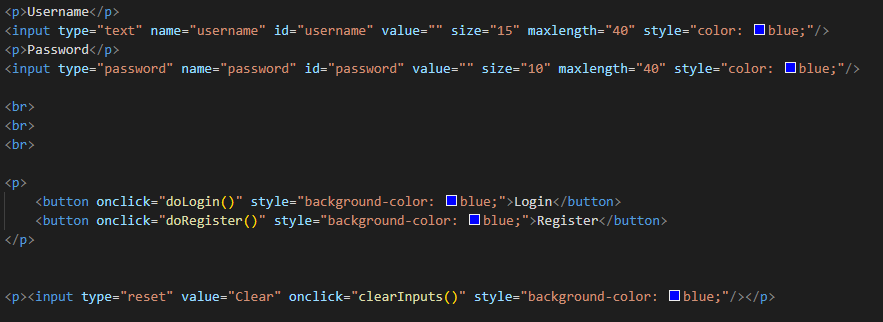
\includegraphics[scale=0.60]{Images_code/4 - html index.png}
        \caption{\label{Estrutura}Organização dos elementos que constituem a aplicação WEB}
\end{figure}

\newpage

Ao clicar no botão “Register”, é invocada a função “doRegister()” em javascript, que se encontra em ./js/login.js. A função envia um /POST ao método doRegister do atributo “acios” (classe Actions) do servidor WEB (app.py) com as credenciais como parâmetros:

\begin{figure}[!hbtp]

        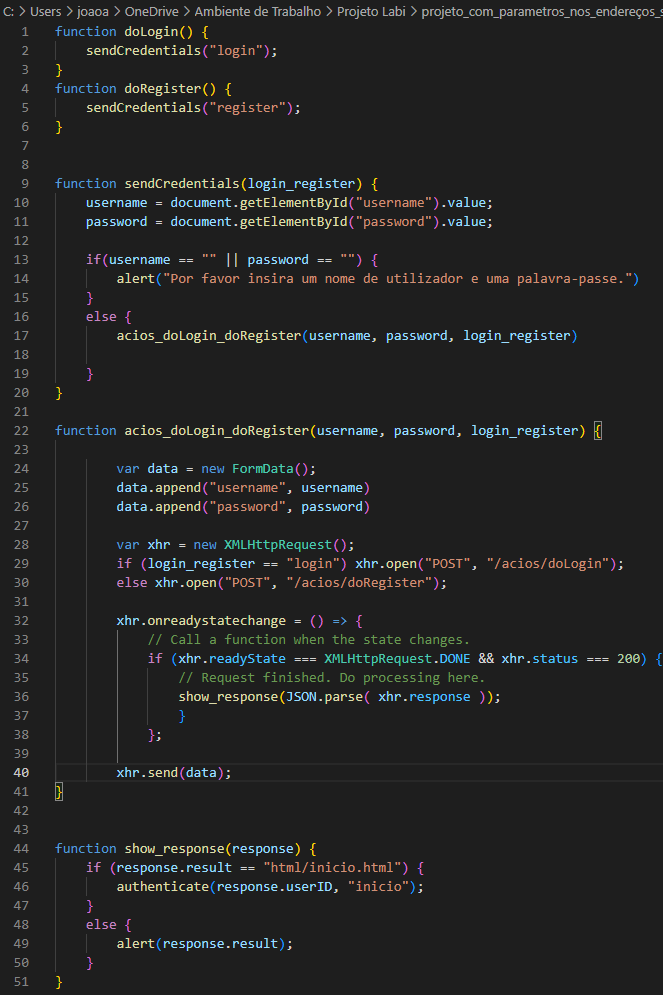
\includegraphics[scale=0.60]{Images_code/5 - js login.png}
        \caption{\label{Estrutura}Função “doRegister()”. Notar que a função que envia o /POST para registo, é a mesma que o faz para o login, havendo um “if” para as separar}
\end{figure}

\begin{figure}[!hbtp]

        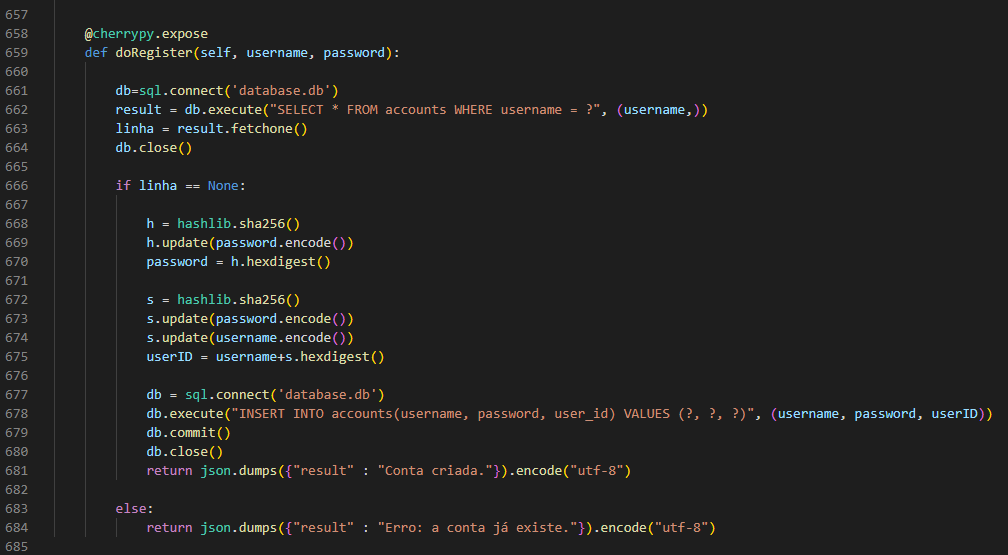
\includegraphics[scale=0.50]{Images_code/6 - app - doRegister.png}
        \caption{\label{Estrutura}Método “doRegister” da classe Actions (atributo .acios da classe Root).}
\end{figure}

Ao receber as credenciais do utilizador, o método verifica, na tabela “accounts” da base de dados, se este nome de utilizador já existe.

\linebreak
\bigskip

Quer exista quer não exista, o método retorna um objeto json a informar a função javascript que fez o POST que já existe, ou não, uma conta com essa nome; a função simplesmente mostra um alerta na página html a mostrar essa precisa informação. No entanto, se não existir essa conta ainda, o método acede à base de dados e cria essa conta (linhas 677-680 do método "doRegister").

\linebreak
\bigskip

Note-se ainda que no campo da password, não é inserida a password que o utilizador escreveu, mas sim uma síntese (sha256) da mesma, e que no campo user\_id, é inserido um valor correspondente à concatenação do nome de utilizador (que é único, e como tal, este campo também vai ser único devido a tal) com a \underline{síntese da síntese} da password. 

\linebreak
\bigskip

Este método de segurança é o que permite que cada utilizador navegue segura e unicamente pela interface (após o login) da aplicação, sendo que no endereço, fica escondida a informação da password (visto que é quase impossível “desfazer” uma síntese sha256, quanto mais uma por cima de outra).

\newpage

	Para o caso de um utilizador fazer login, o processo é muito semelhante, mas não há alteração na base de dados, apenas consulta, e se as credenciais forem válidas, o método doLogin retorna um objeto json que a função .js que fez o POST (linhas 45-46), em vez de mostrar um alerta, autentica o utilizador e envia-o para a pagina de início.



\begin{figure}[!hbtp]

        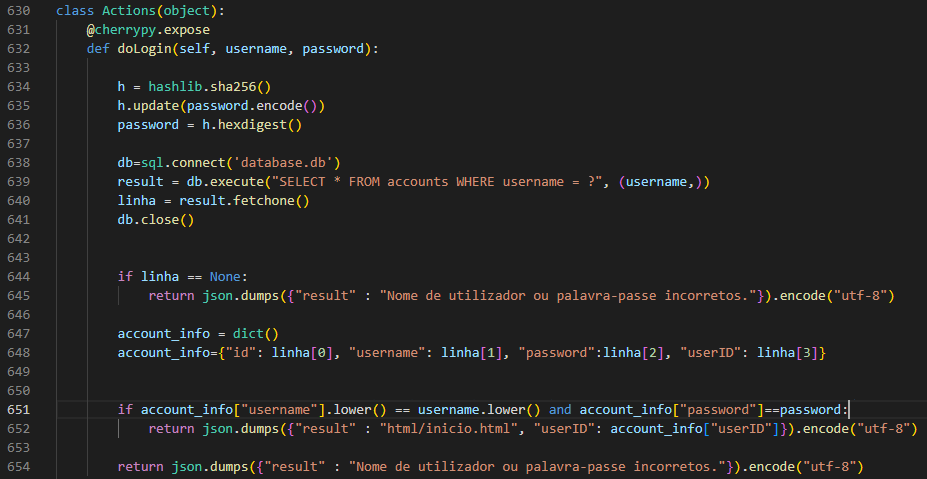
\includegraphics[scale=0.60]{Images_code/7 - login.png}
        \caption{\label{Estrutura}Método “doLogin”.}
\end{figure}


 Depois de autenticado, sempre que um utilizador tentar aceder a uma página html, o parâmetro userID, obtido do campo “user\_id” da tabela “accounts”, será usado para verificar a autenticidade do utilizador, e obter o seu “username” no caso de aceder à página Upload ou clicar numa imagem na página Gallery.

\begin{figure}[!hbtp]

        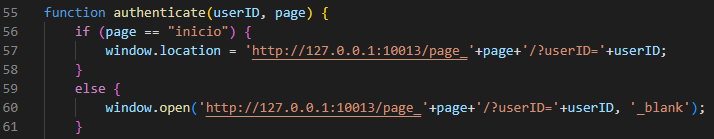
\includegraphics[scale=0.80]{Images_code/8 - js authenticate.png}
        \caption{\label{Estrutura}Função “authenticate”, responsável por (usando um método do servidor) mudar de página, assegurando a identidade do utilizador que o está a fazer. }
\end{figure}

\newpage


 A função “authenticate” usa os mecanismos de uso de endereços do cherrypy, mais concretamente, com o cherrypy.expose, para mudar de página. Cada página tem associado um método cujo nome começa por “page\_” e acaba no nome da página em concreto (por exemplo, “page\_gallery” é o método que permite aceder à página da galeria).

\linebreak
\bigskip
 
	Visto que a pasta onde estão as páginas html não está configurada no cherrypy para ser estática, pelas razões de segurança já referidas, usamos métodos para atingir o mesmo objetivo; sendo que estes métodos precisam de um argumento, o “userID” já falado, único a cada utilizador, para validar a mudança de página. Caso o “userID” passado como parâmetro não esteja na base de dados, o método redireciona o utilizador para a página de login/registo.

\begin{figure}[!hbtp]

        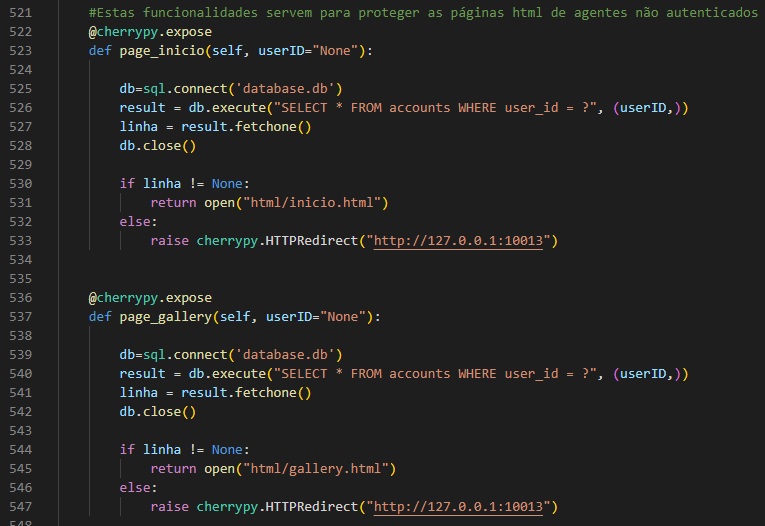
\includegraphics[scale=0.60]{Images_code/9 - app paginas.png}
        \caption{\label{Estrutura}Métodos de acesso às páginas, utilizados pela função “authenticate” explicita na figura 2.6.}
\end{figure}

 Visto isto, passemos à tabela “images”, e como é que o servidor interage com ela, e como é que a interface faz com o que o servidor interaja com ela.

\newpage


\subsection{Tabela images – o que é e como interagir com ela}

A tabela da base de dados que armazena os dados auxiliares de uma imagem na base de dados designa-se images. Os campos desta tabela são: o autor da imagem (author), ou seja o utilizador que carregou a imagem no sistema; o nome que o utilizador lhe atribuiu (name); a data e hora do carregamento da imagem (datetime); e o caminho para a imagem (path), ou seja o diretório onde se encontra o ficheiro. O campo id, como no caso da tabela accounts, representa a chave primária, e é automaticamente incrementado a cada inserção.

\linebreak
\bigskip

	Esta tabela é atualizada a partir do carregamento de imagens por parte do utilizador na página “Upload”. Esta página (html) tem um “input” de imagens, cujo clique invoca a função “uploadPhoto”, que mostra a imagem na página, e guarda os dados (binários, em formato File da classe Blob de javascript) da imagem em si numa variável, para posterior envio num POST ao servidor, caso se clique no botão de envio, que chama a função “uploadImage”.

\linebreak
\bigskip

	Destaca-se ainda função “autofill”, chamada logo quando a página é carregada, que a partir do endereço da página (que contém o “userID” como parâmetro identificador do utilizador), preenche o campo de nome do autor com o nome do utilizador. Este processo não é direto, sendo efetuado um POST ao método “getUsername” do servidor para “converter” o “userID” no “username” respetivo. 

\newpage

\begin{figure}[!hbtp]

        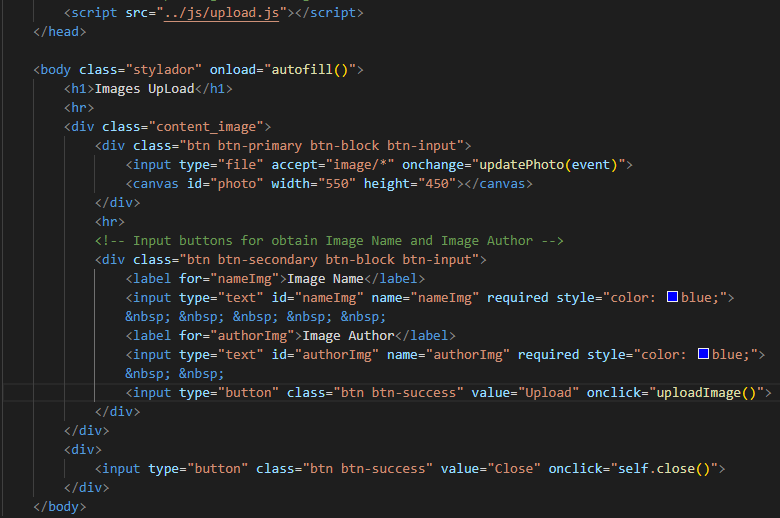
\includegraphics[scale=0.6]{Images_code/9 - html upload.png}
        \caption{\label{Estrutura}Página Upload, em html.}
\end{figure}


\begin{figure}[!hbtp]

        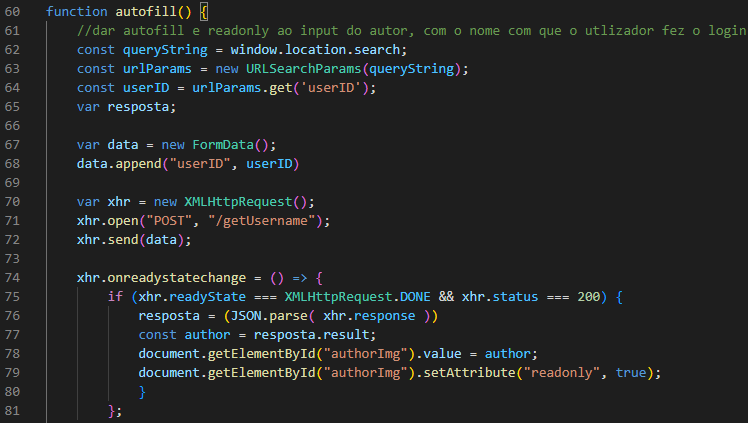
\includegraphics[scale=0.66]{Images_code/9 - js autofill.png}
        \caption{\label{Estrutura}Função “autofill”, que a partir do parâmetro “userID” do endereço da página, preenche o campo de nome do autor com o nome do utilizador.}
\end{figure}



\begin{figure}

        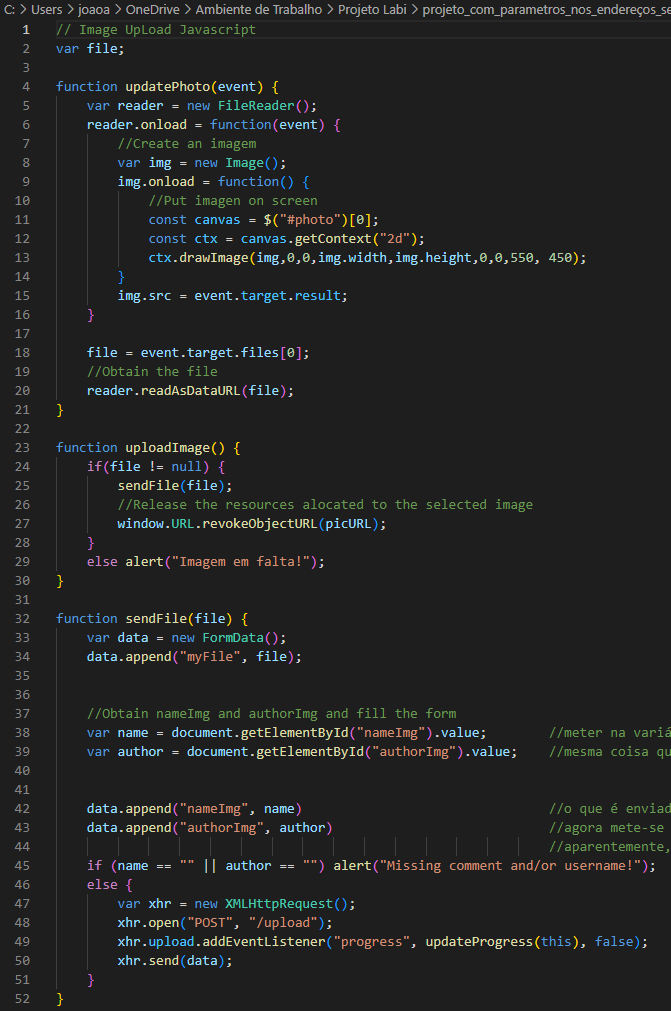
\includegraphics[scale=0.63]{Images_code/9 - js upload.png}
        \caption{\label{Estrutura}Funções “updatePhoto” (que carrega a imagem na página e guarda os dados numa variável) e “uploadImage”, que envia o POST ao servidor.}
\end{figure}




\newpage

Do lado do servidor, temos o método “upload”, responsável por guardar a imagem em si no servidor (com um caminho obtido a partir da junção do caminho da pasta onde se encontra o servidor, mais a pasta “uploads/”, mais o resultado da síntese da imagem) e fazer o registo das suas informações (nome, autor, data, caminho) na base de dados, e o método “getUsername”, que retorna o “username” ao qual o parâmetro de entrada “userID” está associado.

\linebreak

\begin{figure}[hbp]

        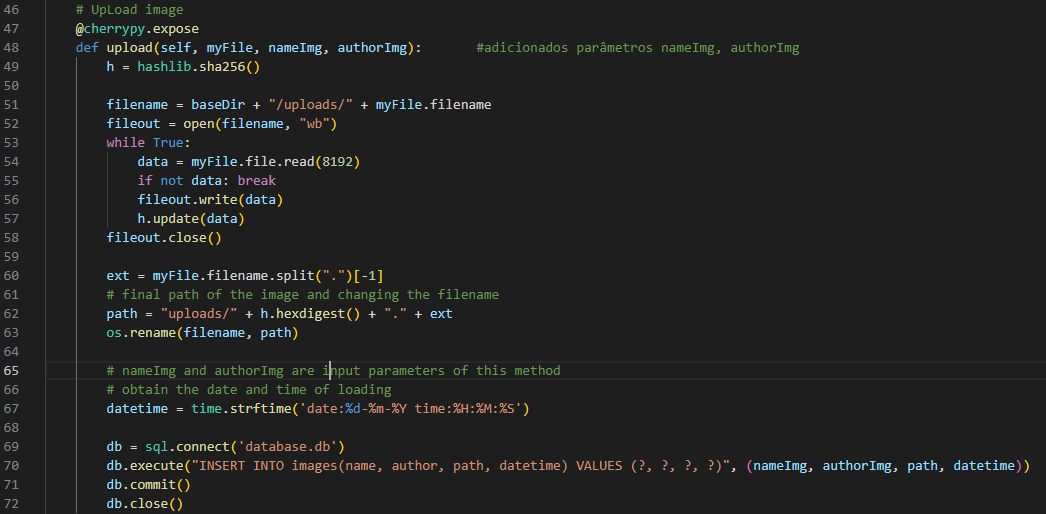
\includegraphics[scale=0.50]{Images_code/9 - app upload.png}
        \caption{\label{Estrutura}Método “upload”. }
\end{figure}

\begin{figure}[hbp]

        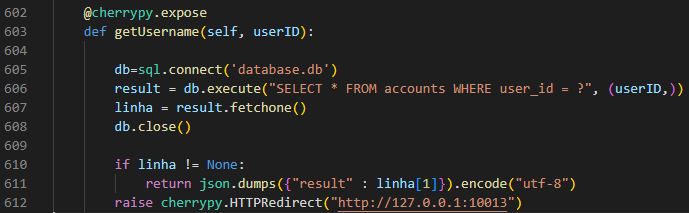
\includegraphics[scale=0.75]{Images_code/9 - app getusername.png}
        \caption{\label{Estrutura}Método “getUsername”. }
\end{figure}

 Esta descrição cobre os pontos essenciais da funcionalidade de carregamento de imagens. Passemos agora à funcionalidade de visualização de imagens, na página Gallery, que ainda usa a tabela “images” da base de dados.

 \newpage
 
    A página Gallery mostra todas as imagens carregadas no servidor (em concreto, as que foram carregadas através da página Upload), ordenadas pelo seu nome (nome que o autor deu, e não o de síntese, e que aparece sobre cada imagem, juntamente com o nome do autor), e permite a filtragem das mesmas pelo nome do autor (note-se que pode-se usar sintaxe sql “\%autor” para obter matches parciais; note-se ainda que todo o nosso código sql foi feito de maneira a evitar sql injection).

 \begin{figure}[hbp]

        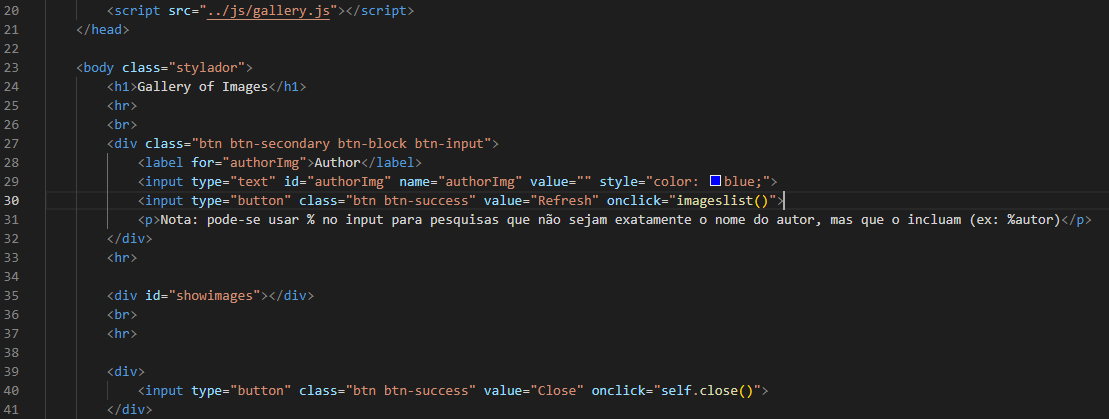
\includegraphics[scale=0.5]{Images_code/10 - html gallery.png}
        \caption{\label{Estrutura}Página Gallery, em html}
\end{figure}


 Note-se que o div com id=”showimages” começa vazio; ele é populado pela função “showimage”, chamada pela “imageslist”, que faz um POST ao método “list” do servidor (com parâmetro de autor), e a partir da resposta deste (que contém os caminhos necessários para representar as imagens na página html através do atributo “src” dos elementos “img”, e que também contém as informações de autor e nome, todas obtidas a partir da tabela “images” da base de dados), itera sobre cada dicionário de informações de imagens recebido, e faz “append” dos elementos (“img” e “h3”) criados nesse div.

 \newpage



\begin{figure}[!hbtp]
        \centering
        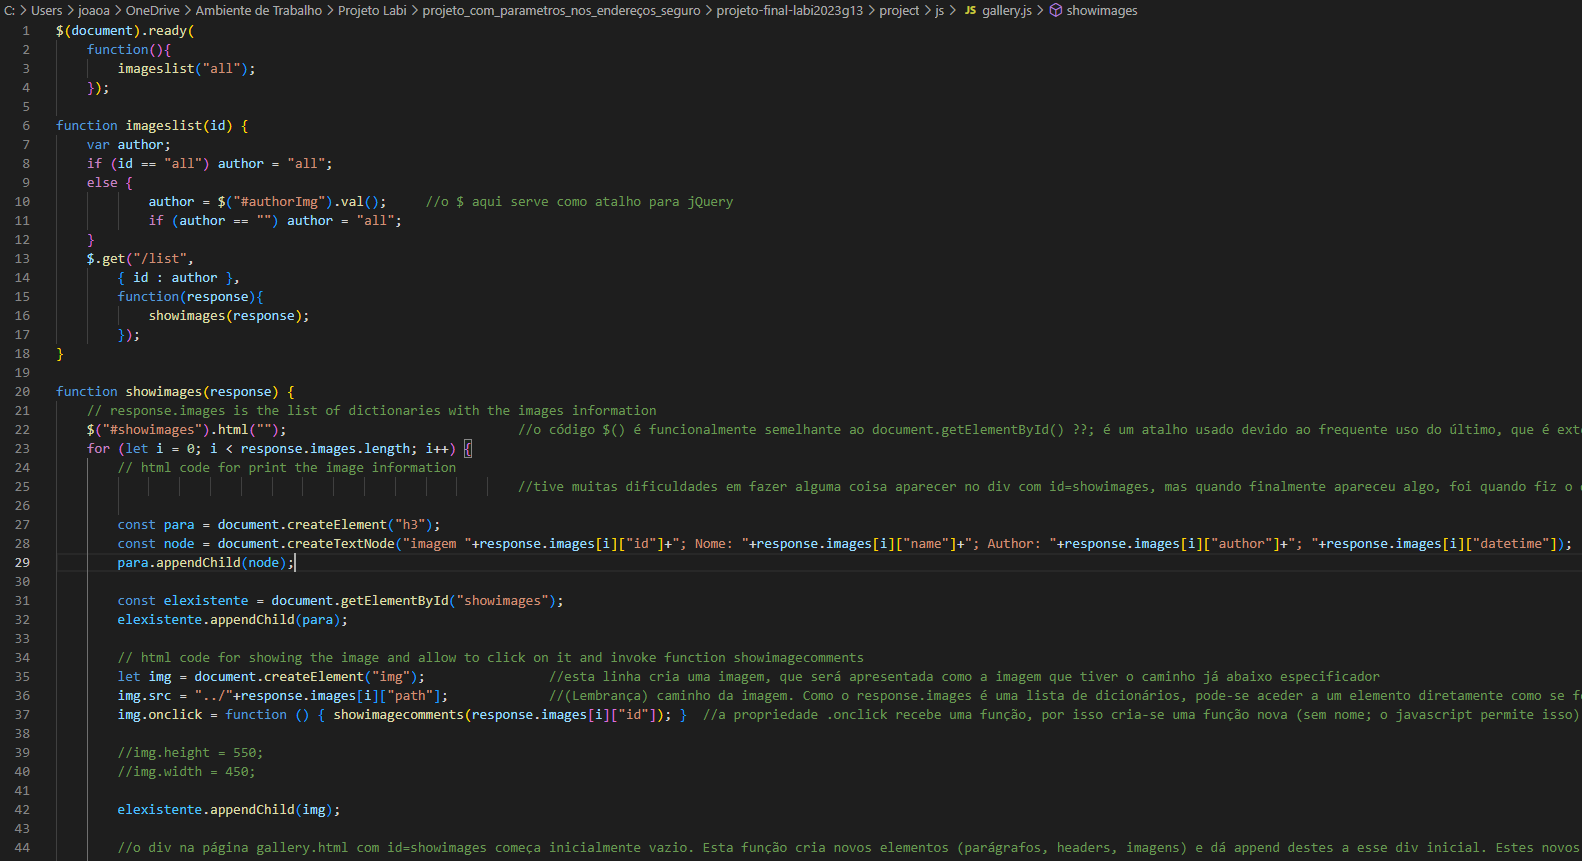
\includegraphics[scale=0.32]{Images_code/10 - js gallery.png}
        \caption{\label{Estrutura}Função “imagelist”, que faz um POST ao servidor com a informação de autor a filtrar, e a função “showimages”, que a partir da resposta do servidor (que depende também da base de dados), adiciona as imagens, os seus nomes, e os nomes dos seus autores à página html.}
\end{figure}

\begin{figure}[!hbtp]
        \centering
        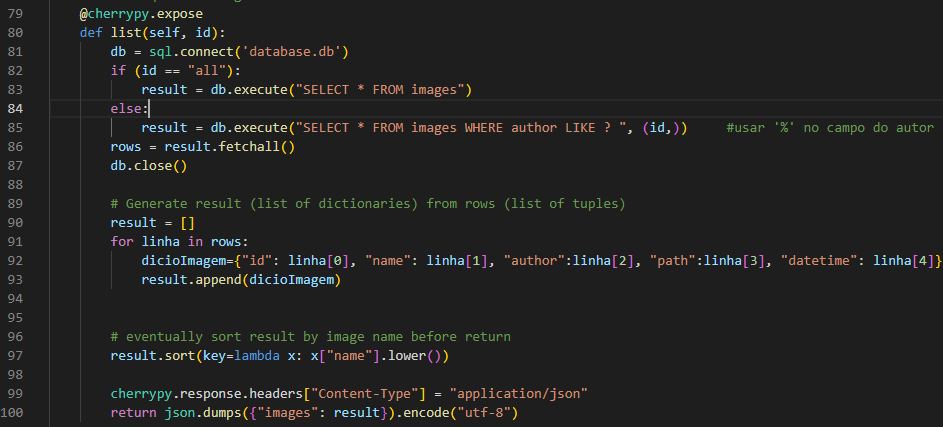
\includegraphics[scale=0.55]{Images_code/10 - app list.png}
        \caption{\label{Estrutura}Método “list” do servidor, que procura na tabela “images” da base de dados as informações das imagens cujo autor corresponde ao parâmetro indicado, e retorna essas informações, ordenadas, numa lista de dicionários em formato json.}
\end{figure}

\newpage


 Esta descrição tenta demonstrar o essencial sobre a implementação da funcionalidade de visualizar imagens, mas nesta mesma página da Galeria, pode-se aceder a outra funcionalidade: a de ver os comentários e gostos/desgostos de uma imagem em particular. Na Fig16, linha 37, demonstra-se a atribuição de um evento “onclick” a cada imagem. Este evento permite que, ao clicar numa imagem, seja aberta uma nova página, dedicada a esta nova funcionalidade.

\begin{figure}[!hbtp]
        \centering
        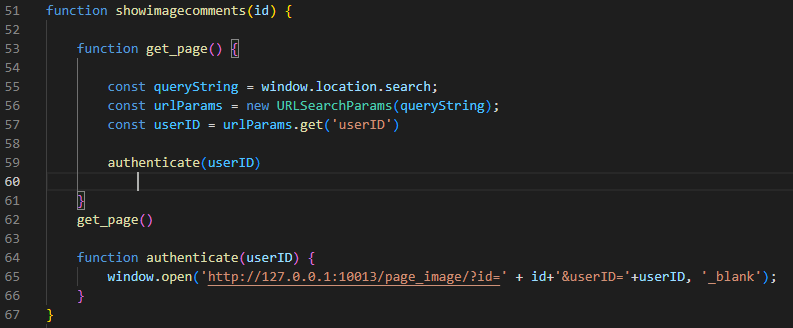
\includegraphics[scale=0.60]{Images_code/10 - js gallery image.png}
        \caption{\label{Estrutura}Definição da função “showimagecomments”.}
\end{figure}

\bigskip

 A função “showimagecomments” que é atribuída a cada imagem mostrada na galeria, confere acesso à funcionalidade de ver e fazer comentários e gostos e desgostos à imagem. 

 \linebreak
 \bigskip
 
 Para este efeito, ela recebe um parâmetro de id, correspondente ao id da imagem selecionada na tabela “images” da base de dados (onde está o seu caminho, que é essencial para a sua visualização), e acede ao método “page\_image” do servidor (GET) para obter a página image.html.

 \newpage

\begin{figure}[!hbtp]
        \centering
        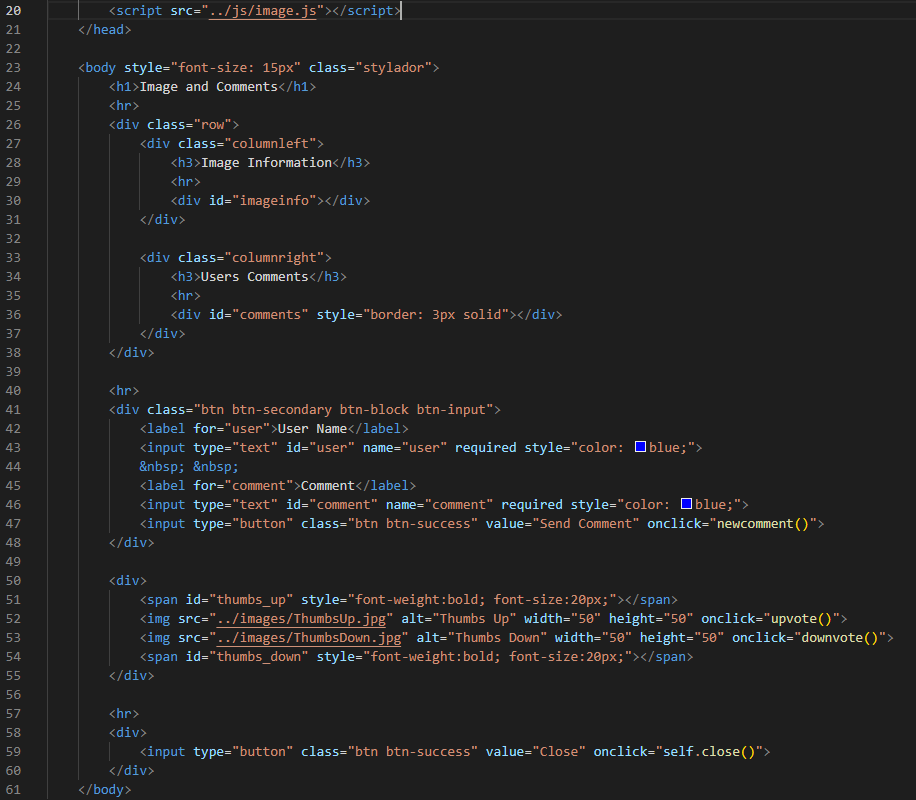
\includegraphics[scale=0.60]{Images_code/11 - html image.png}
        \caption{\label{Estrutura}Página Image, em html.}
\end{figure}


 Embora não seja aqui mostrado na página html, na função javascript respetiva, o id da imagem é obtido logo a partir do parâmetro “id” do endereço assim que a imagem é carregada (obtendo-se assim um parâmetro essencial para obter o caminho, o nome, e o autor da imagem, bem como a data e a hora na qual foi carregada).
 
	

 \newpage

\begin{figure}[!hbtp]
        \centering
        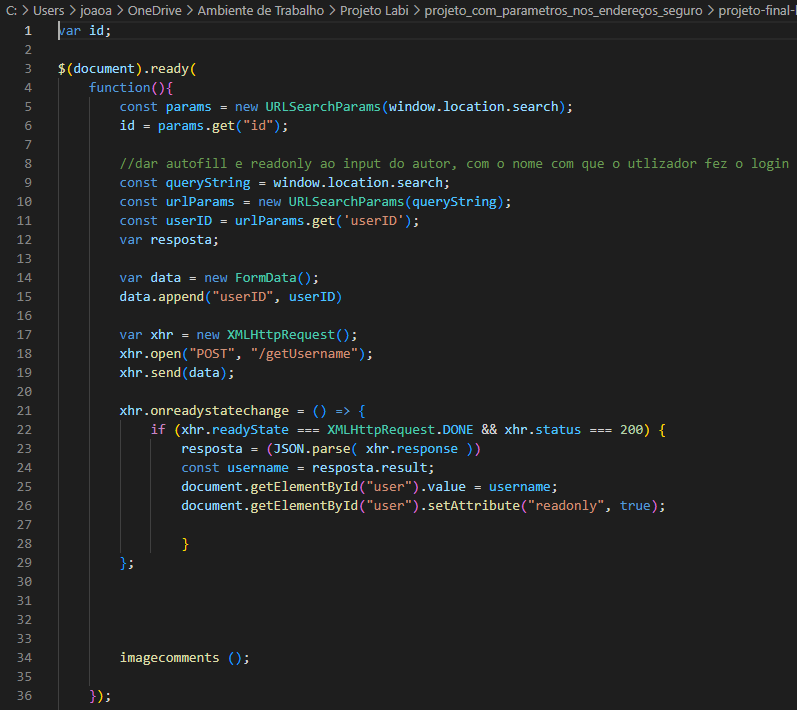
\includegraphics[scale=0.60]{Images_code/11 - js image.png}
        \caption{\label{Estrutura}Função javascript imagem.js; função “onload” da página respetiva.}
\end{figure}

Também é obtido o “username” do utilizador a partir do “userID” no endereço, de maneira semelhante à que já foi descrita, e que é usado para preencher o campo de autor de comentário, que corresponde ao elemento com id=”user” na imagem acima.

\newpage

 \subsection{Tabelas comments e votes – como é que são usadas}

 As informações sobre os comentários e votos da imagem selecionada são obtidos a partir da tabela “comments” da base de dados, que é feito a partir da função “imagecomments”, que faz um POST ao método “comments” do servidor, cuja resposta é manipulada pela função “showimageandinfo”, de modo a criar os elementos html necessários para mostrar todos os comentários e votos obtidos na página.

\begin{figure}[!hbtp]
        \centering
        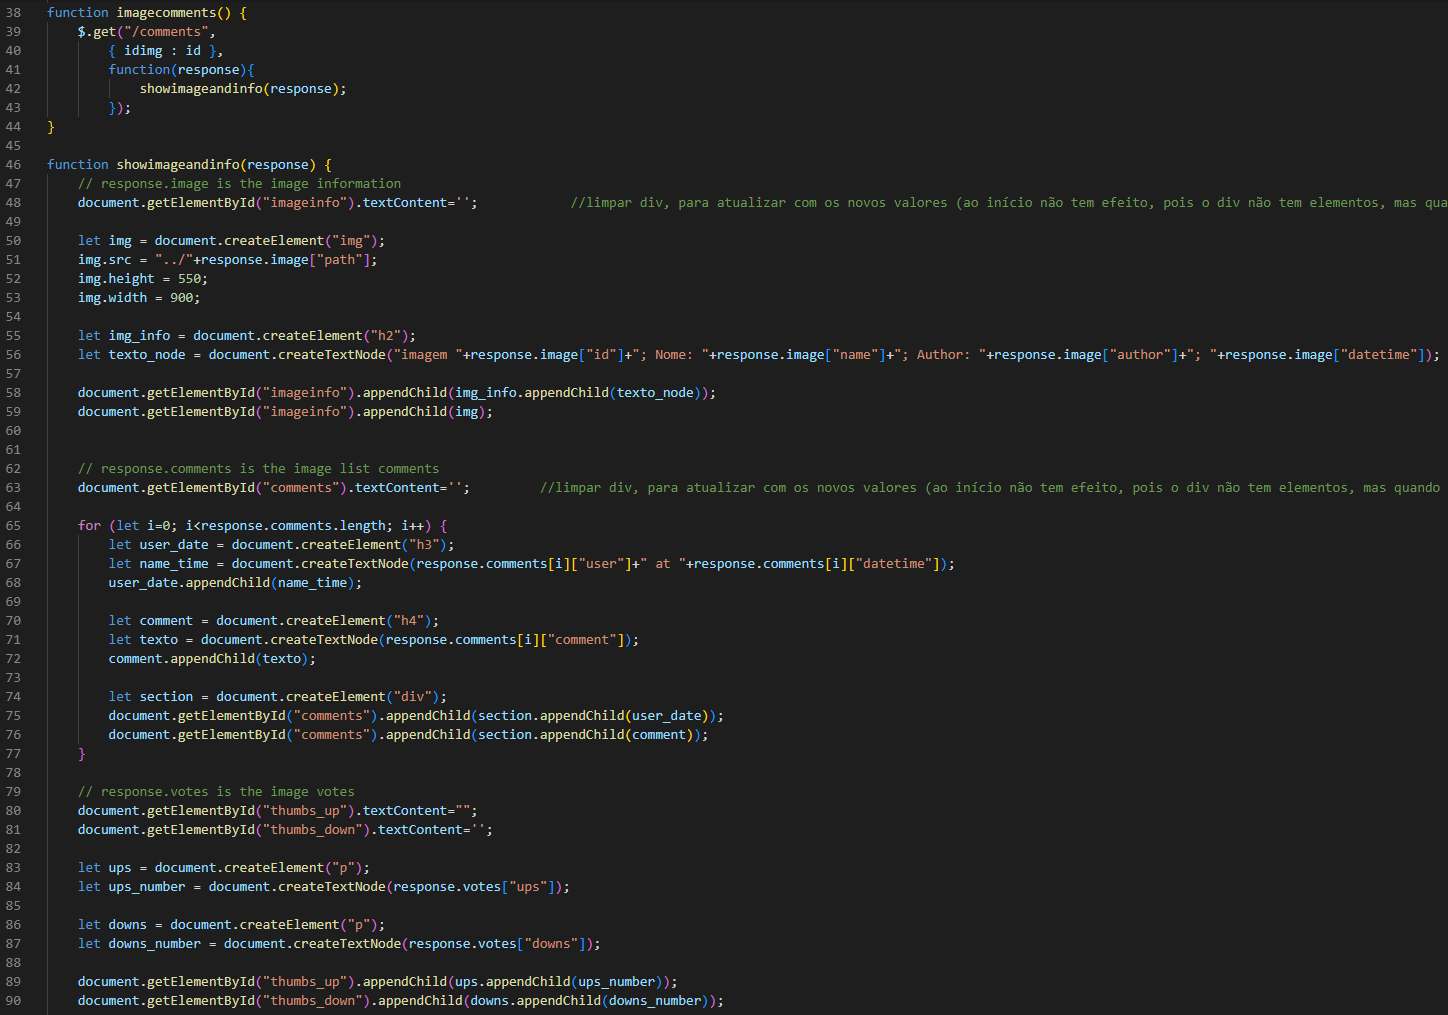
\includegraphics[scale=0.40]{Images_code/11 - js image 2.png}
        \caption{\label{Estrutura}Funções “imagecomments” e “showimageinfo”.}
\end{figure}

\bigskip

 Do lado do servidor, o método “comments” procura em 3 tabelas distintas da base de dados (images, votes e comments) as informações necessárias para que se possa visualizar a imagem (com o seu caminho), o seu nome, o seu autor, a hora e data a que foi submetida, bem como as informações de todos os comentários e gostos e desgostos feitos relativamente a esta imagem.
 

\newpage
 
	Só há uma imagem a ser representada, e os votos são aglomerados em valores totais (não é mostrado quem meteu gosto ou desgosto, simplesmente se mostra o valor total de cada métrica), pelo que um dicionário para cada é suficiente para representar essa informação. Os comentários podem ser diversos, e importa saber quem os fez, por isso é necessária uma lista de dicionários para representar esta informação.

 \linebreak
 \bigskip
 
	Toda ela é posteriormente devolvida num objeto json, que é extensivamente usado pela função “showimageandinfo” para meter em html estes dados.


 \begin{figure}[!hbtp]
        \centering
        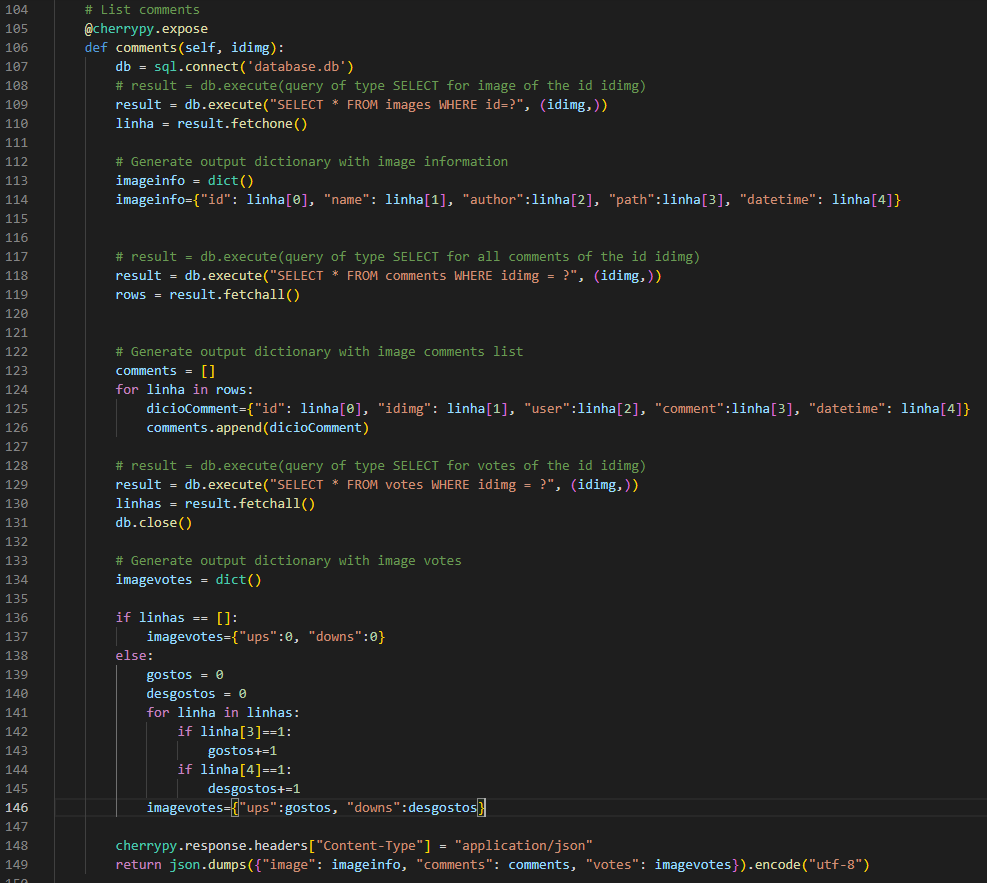
\includegraphics[scale=0.50]{Images_code/11 - comments votes.png}
        \caption{\label{Estrutura}Método “comments”.}
\end{figure}

\newpage


 Para terminar esta secção da funcionalidade de apreciação da foto, não basta descrever como é que se pode ver essa informação, mas também como é que se pode adicionar comentários e gostos à imagem selecionada.

 \linebreak
 \bigskip
 
	A página html tem campos de texto para escrever comentários (o campo de autor é automaticamente preenchido, como já referido), com o devido botão de submeter, e tem também pequenas imagens que representam os likes e dislikes, que ao carregar neles, faz-se gosto e desgosto, respetivamente. Carregar novamente nestes botões, retira o gosto ou desgosto feito, conforme é usual acontecer em aplicações que permitem esta funcionalidade (como o Facebook e o Instagram).

\begin{figure}[!hbtp]
        \centering
        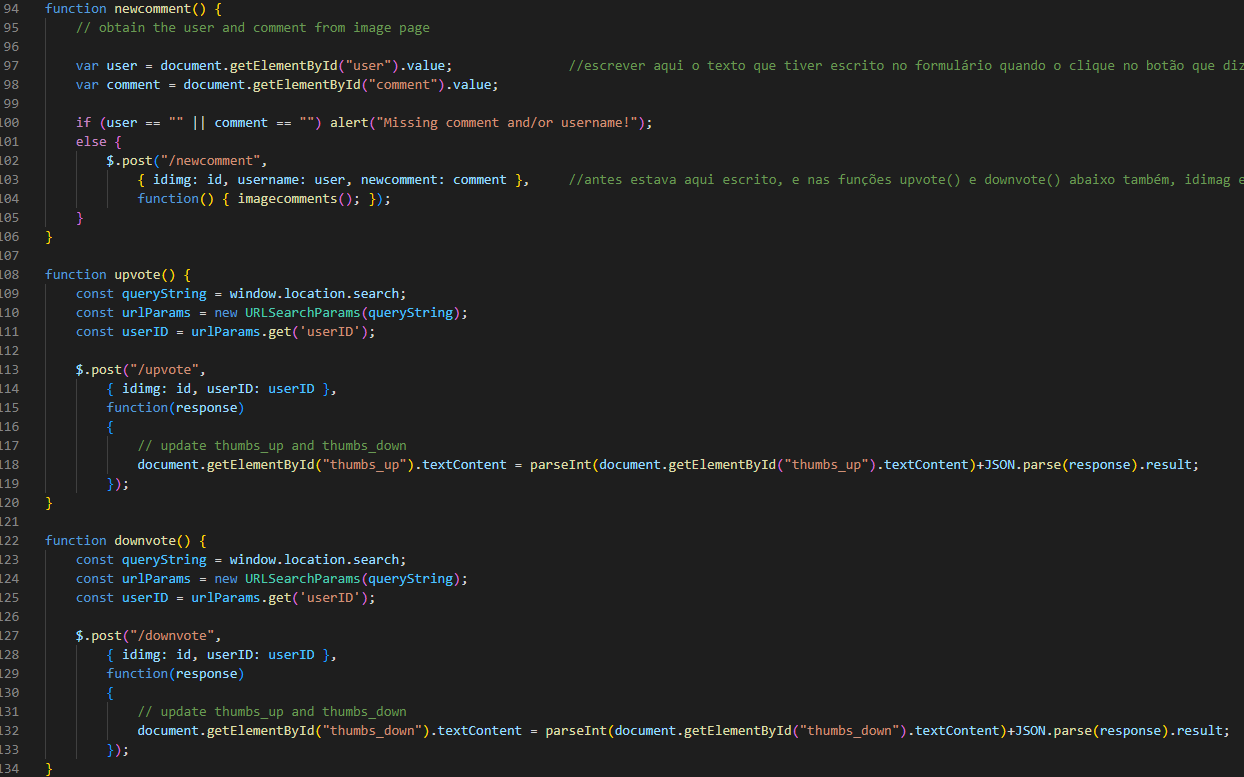
\includegraphics[scale=0.46]{Images_code/11 - js image 3.png}
        \caption{\label{Estrutura}Funções “newcomment”, “upvote” e “downvote”.}
\end{figure}


 Sempre que é submetido um novo comentário (e é invocada a função “newcomment”, que faz POST  ao método com o mesmo nome no servidor), a div que os mostra é apagada de todo o seu conteúdo, pois será feita uma nova chamada à função “imagecomments”, e posteriormente “showimageandinfo”, que já foram descritas, para mostrar todos os comentários.

 \newpage


 \begin{figure}[!hbtp]
        \centering
        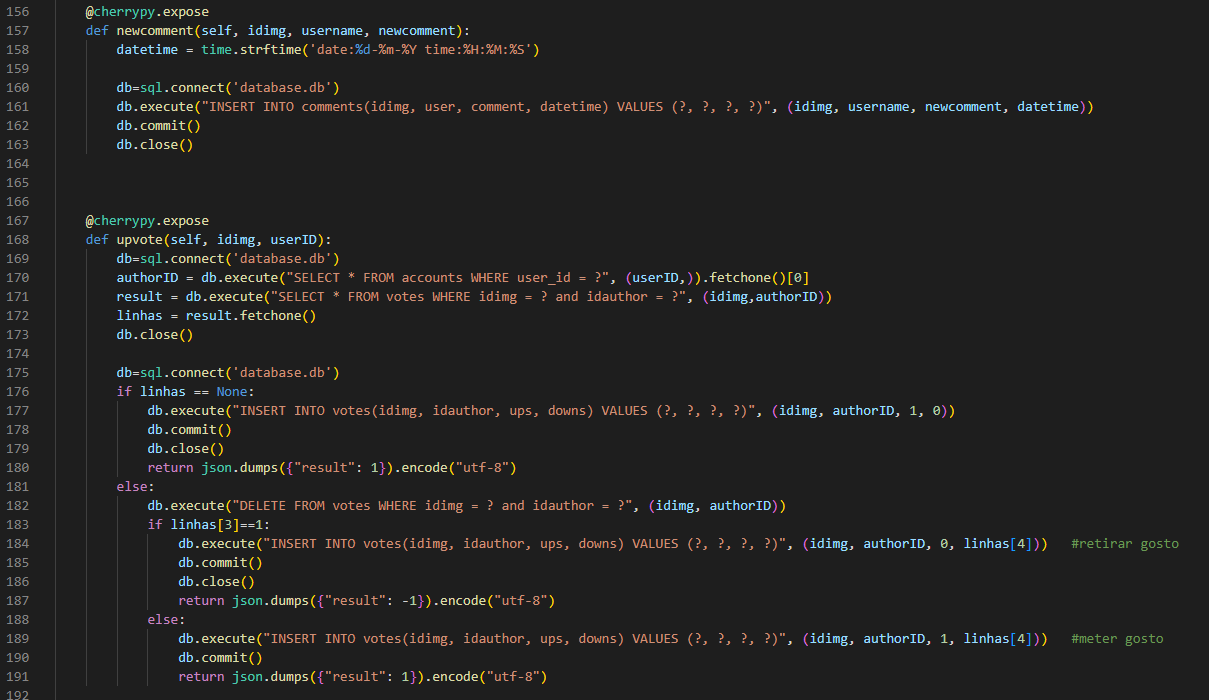
\includegraphics[scale=0.46]{Images_code/11 - newcomments.png}
        \caption{\label{Estrutura}Métodos “newcomment” e “upvote” (o método “downvote” é muito semelhante ao método "upvote", só que atualiza os desgostos em vez dos gostos).}
\end{figure}



 \linebreak
 \bigskip
 \bigskip
 \bigskip
 Para concluir a secção da metodologia, demonstremos agora como implementámos a única funcionalidade que ainda não explicitámos (e a única que não faz uso da base de dados): a manipulação de imagens

 \newpage
\subsection{Manipulação de imagens}

A funcionalidade de manipulação de imagens da nossa aplicação é muito complexa, mesmo não usando a base de dados. A base de dados não é usada, porque as imagens que o utilizador pretender manipular, são carregadas a partir do seu computador/dispositivo, e estas já contém os dados necessários para que os nossos métodos de manipulação de imagem funcionem.

\linebreak
 \bigskip

 
	O utilizador, ao carregar uma imagem na página Image Manipulation, e ao submeter a imagem para manipulação, faz com que esta, caso seja validada a par com os outros “inputs” pedidos pelo método de manipulação escolhido, faz com que a imagem seja guardada na pasta ./tmp da aplicação, para que os seus dados possam ser usados pelos métodos do servidor (que são definidos num ficheiro python complementar, e importados e usados no programa principal em si) para que a manipulação da imagem ocorra. Caso a manipulação seja bem sucedida, a imagem resultante também é guardada na pasta ./tmp, e é mostrada na página html através de funções javascript.

 \linebreak
 \bigskip
 
	Caso o utilizador goste da imagem que manipulou, pode simplesmente guardá-la a partir da página ao clicar com o botão direito (ou usando outro método que alcance o mesmo resultado) e escolher “Guardar imagem”. Se posteriormente pretender com que esta imagem manipulada seja mostrada na página da Galeria, pode carregá-la na página Upload, mas não é obrigado a carregar primeiro a imagem original que deseja manipular (ou imagens, caso o método de manipulação o peça) no servidor (embora o possa fazer à vontade).

 \linebreak
 \bigskip
 
	Ao entrar na página Image Manipulation, encontram-se 2 secções distintas, lado a lado: uma, do lado esquerdo, para escolher uma imagem, e outra, do lado direito, que é usada para mostrar a imagem manipulada.

 \linebreak
 \bigskip

	Mas para manipular a imagem, é preciso escolher um método, a partir duma lista opções sob a forma de elemento “select” que se encontra no centrado com a página, juntamente com o botão de submeter, mas abaixo das 2 secções mencionadas acima. Ao selecionar um método de manipulação, podem aparecer, conforme o método, outros “inputs” para o utilizador escolher/preencher abaixo do botão de submeter, ou pode até aparecer, do lado esquerdo, abaixo da secção de “input” da imagem original a escolher, outro “input” de imagem para o utilizador usar.

 \newpage
 \begin{figure}[!hbtp]
        \centering
        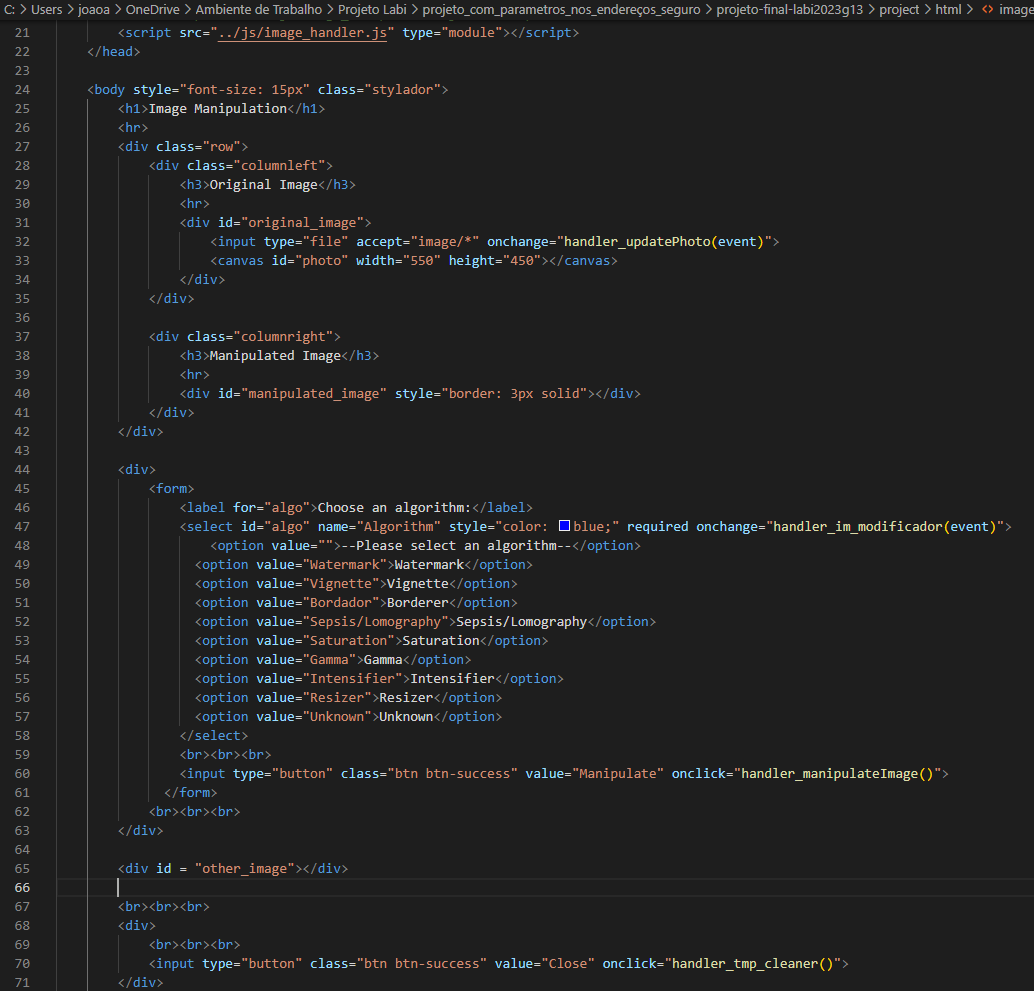
\includegraphics[scale=0.53]{Images_code/12 - image manipulation html.png}
        \caption{\label{Estrutura}Página de Image Manipulation em html.}
\end{figure}

 
Destaca-se aqui o elemento “div” com id=”original\_image”, dentro dum outro “div” com class=”columnleft”, o elemento “div” com id=”manipulated\_image”, dentro dum “div” com class=”columnright”,  e o elemento “div” vazio com id=”other\_image”.

\linebreak
 \bigskip
 
	Os dois primeiros “divs” servem para carregar e mostrar a imagem original, e para mostrar a imagem manipulada, respetivamente. O outro “div” é usado pelos métodos de manipulação para colocarem nele os “inputs” que forem precisos.

\linebreak
 \bigskip
 
O primeiro método de manipulação de imagem que fizemos foi o “watermark”, que adiciona uma imagem noutra, e que coloca neste último “div” um outro “div”, com class=”columnleft”, que em si terá um “input” de imagem, semelhante ao que se encontra no primeiro “div” com id=”original\_image”.


 

 \begin{figure}[!hbtp]
        \centering
        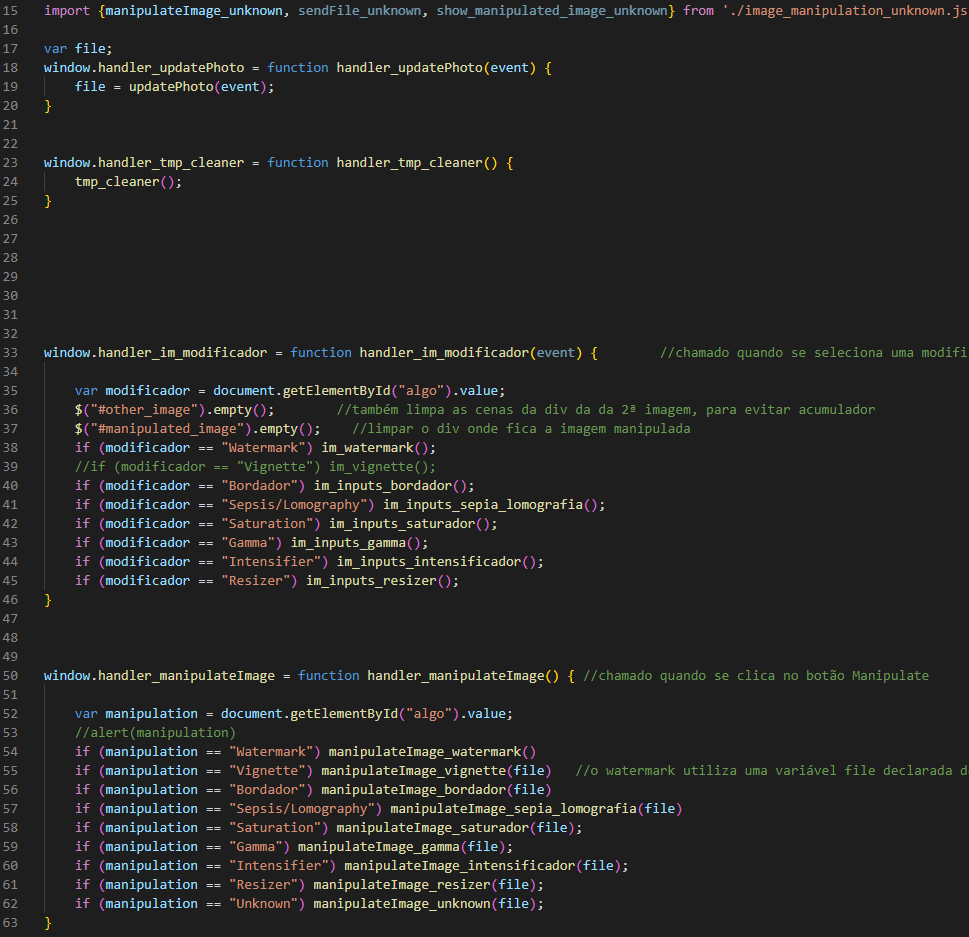
\includegraphics[scale=0.52]{Images_code/12 - image manipulation js handler.png}
        \caption{\label{Estrutura}Script "image\_hander.js".}
\end{figure}


Devido à grande quantidade de métodos de manipulação que foram feitos (estão presentes 9 no "select" da imagem 2.23, mas alguns destes, como a "Sepsis/Lomography", o "resizer", e o "Unknown", contém na verdade 2, 4, 3 e métodos diferentes, respetivamente), decidiu-se criar um ficheiro javascript para definirem-se as funções necessárias para cada um desses métodos listados, funções essas que são posteriormente importadas para um ficheiro javascript chamado "image\_handler.js", que simplesmente delega as funcionalidades pretendidas para as funções que foram importadas. Isto evita que haja um único "hiper-script" com milhares de linhas de código de todas as funções precisas.

\newpage

Quando um método é escolhido, os conteúdos das “divs” correspondentes à imagem manipulada e aos “inputs” específicos de cada método, são apagados, de modo a dar lugar aos novos conteúdos a serem gerados pelo método escolhido.

\linebreak
 \bigskip
 
Devido à grande quantidade de métodos de manipulação de imagens que fizemos, explicitaremos apenas como implementámos 2 métodos: a “watermark”, e o “bordador”. Todos os métodos têm nomes pelos quais se pode inferir a manipulação que fazem, com a exceção propositada do “unknown”, cujo propósito é surpreender o utilizador com uma manipulação de imagem que este não espere (ou pelo menos, criar e satisfazer nele a curiosidade de saber o que este método faz ao certo).

\linebreak
 \bigskip
 
	Começemos pela “watermark”. Quando este método é escolhido, a “div” com id=”other\_image”, correspondente aos “inputs” específicos de cada método, tem os seus conteúdos inicialmente apagados, e é logo populada por um outro “div” (chamado “divs”), com class=”columnleft”, que fica logo abaixo do “div” da escolha de imagem original. Este novo “div” é em si populado por um “input” de imagem, que permite ao utilizador escolher a imagem que quer adicionar como marca de água à imagem original, e por um elemento “canvas”, que é usado para mostrar na página html a imagem escolhida (à imagem do que ocorre com o “div” com id=”original\_image” que está definido na página html).

 \linebreak
 \bigskip
 
	Como já foi referido, o utilizador escolhe ambas as imagens do seu computador pessoal, para que não tenha que as carregar primeiro na galeria (o que poderia ser frustrante se no final não gostasse da imagem manipulada, se é que é possível manipulá-las).

 \linebreak
 \bigskip
 
	Além disso, também é adicionado ao “div” com id=”other\_image” (e não ao “div” alinhado à esquerda que é “appended” nele) um outro “div” (chamado “divsFator”) com um “input” numérico, em que o utilizador tem de inserir um fator de transparência da imagem de marca de água (tem de ser um valor decimal entre 0 e 1, caso contrário, é apresentado um “alert” de erro).

\linebreak
 \bigskip

 	Segue-se na próxima página o código da função que cria e distribui estes elementos.

  \newpage


\begin{figure}[!hbtp]
        \centering
        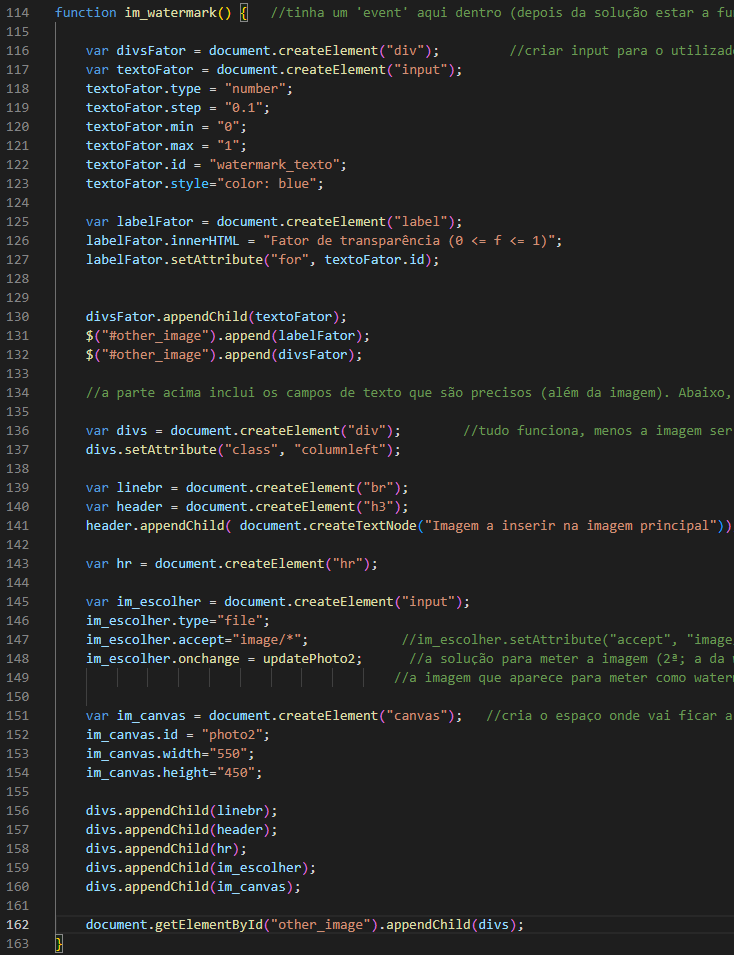
\includegraphics[scale=0.7]{Images_code/12 - image manipulation js watermark im_watermark.png}
        \caption{\label{Estrutura}Função "im\_watermark".}
\end{figure}

\newpage



    	As funções que permitem visualizar a imagem original escolhida e guardar os seus dados (“updatePhoto”), visualizar a imagem escolhida como marca de água e guardar os seus dados (“updatePhoto2”), bem como a função que ocorre ao clicar no botão submeter (que no método “watermark”, é a função “manipulateImage\_watermark”) e a função que mostra a imagem manipulada (caso ela seja manipulada com sucesso) na “div” alinhada à direita (função “show\_manipulated\_image”), são mostradas de seguida.

    \linebreak
 \bigskip

\begin{figure}[!hbtp]
        \centering
        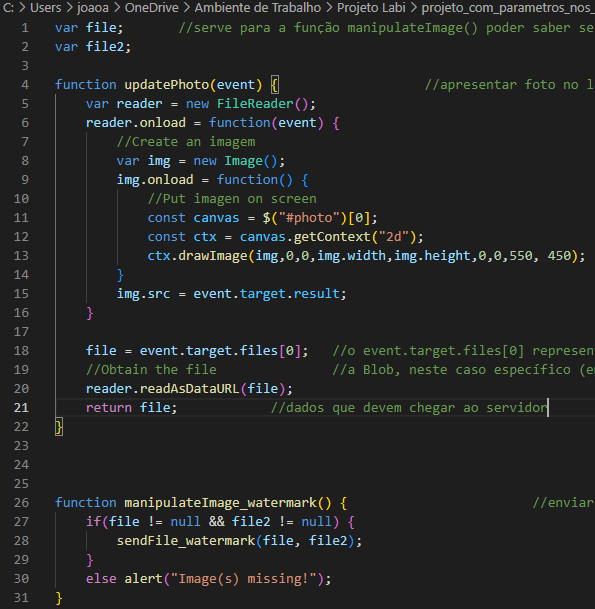
\includegraphics[scale=0.85]{Images_code/12 - image manipulation js watermark uploadPhoto e manipulateImage_watermark.png}
        \caption{\label{Estrutura}Funções "updatePhoto" e "manipulateImage\_watermark".}
\end{figure}




\newpage

\begin{figure}[!hbtp]
        \centering
        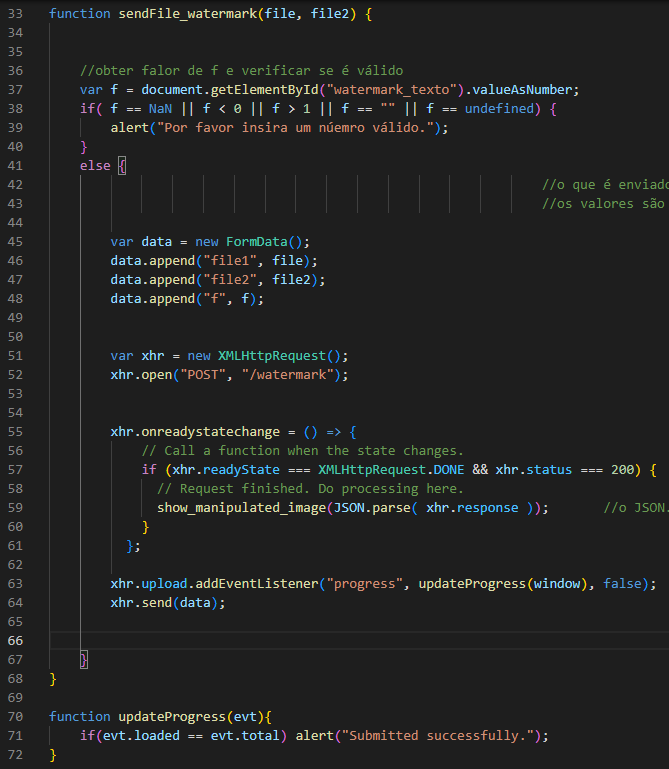
\includegraphics[scale=0.81]{Images_code/12 - image manipulation js watermark sendfile_watermark.png}
        \caption{\label{Estrutura}Função "sendFile\_watermark", que é chamada pela função mostrada acima "manipulateImage\_watermark".}
\end{figure}


\newpage

\begin{figure}[!hbtp]
        \centering
        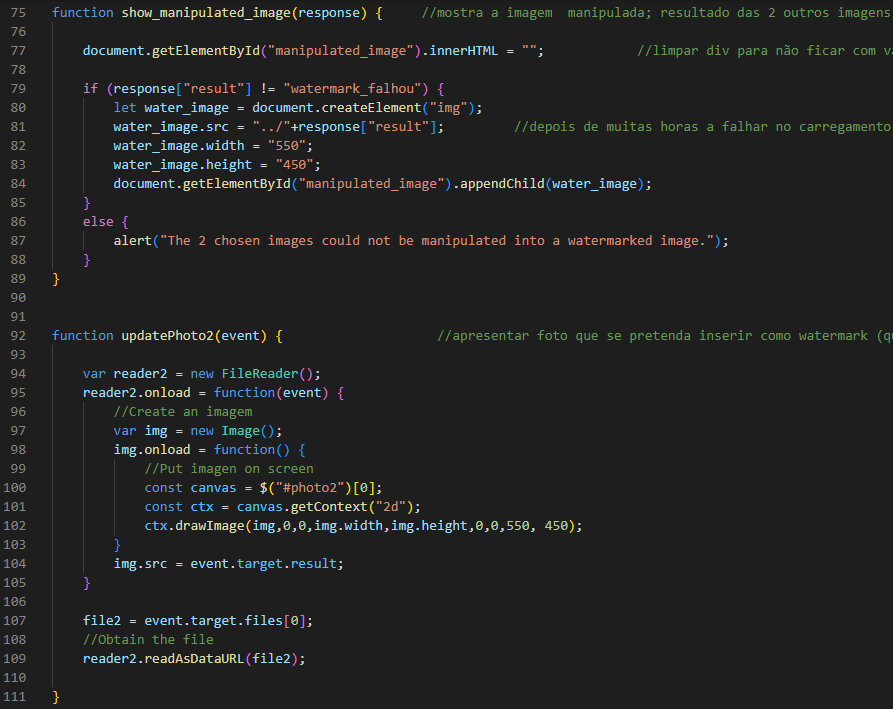
\includegraphics[scale=0.6]{Images_code/12 - image manipulation js watermark showmanipulatedImage e updatePhoto2.png}
        \caption{\label{Estrutura}Funções "show\_manipulated\_image", e "uploadPhoto2".}
\end{figure}

     \linebreak
 \bigskip

 Vejamos agora como é que os dados das imagens e do fator de transparência são usados no servidor, após serem enviados para este a partir do POST que se encontra implementado na função "sendFile\_watermark", mostrada na figura 2.27.
\linebreak
 \bigskip
 O método "watermark" começa por validar o fator de transparência. Se este não representar um valor válido, é retornado um objeto json com uma mensagem de erro para a função "show\_manipulated\_image" (que só mostra a imagem caso seja retornado um objeto com um caminho válido da imagem manipulada no servidor).
 \linebreak
 \bigskip
 Caso seja validado com sucesso o fator de transparência, o método guarda ambas as imagens na pasta ./tmp, e verifica se a manipulação desejada é possível (isto é, verifica se a imagem da marca de água tem dimensões "height" e "width" menores que a imagem princial, através do método "watermark\_positions" importado do ficheiro auxiliar). Se não for, é devolvido a mesma mensagem de erro acima. Se for, então o método procede para a manipulação da imagem (através dum método também chamado "watermark", mas que é proveniente do módulo correspondente ao ficheiro auxiliar, onde todos os métodos de processamento de imagem estão definidos), guardando-a também na pasta ./tmp (sempre com nomes de imagem sintetizados), e devolve o caminho dessa imagem para que a função "show\_manipulated\_image" possa criar um elemento "html" com atributo "src" igual a esse caminho no servidor, o que resulta na visualização da imagem na página html.


\begin{figure}[!hbtp]
        \centering
        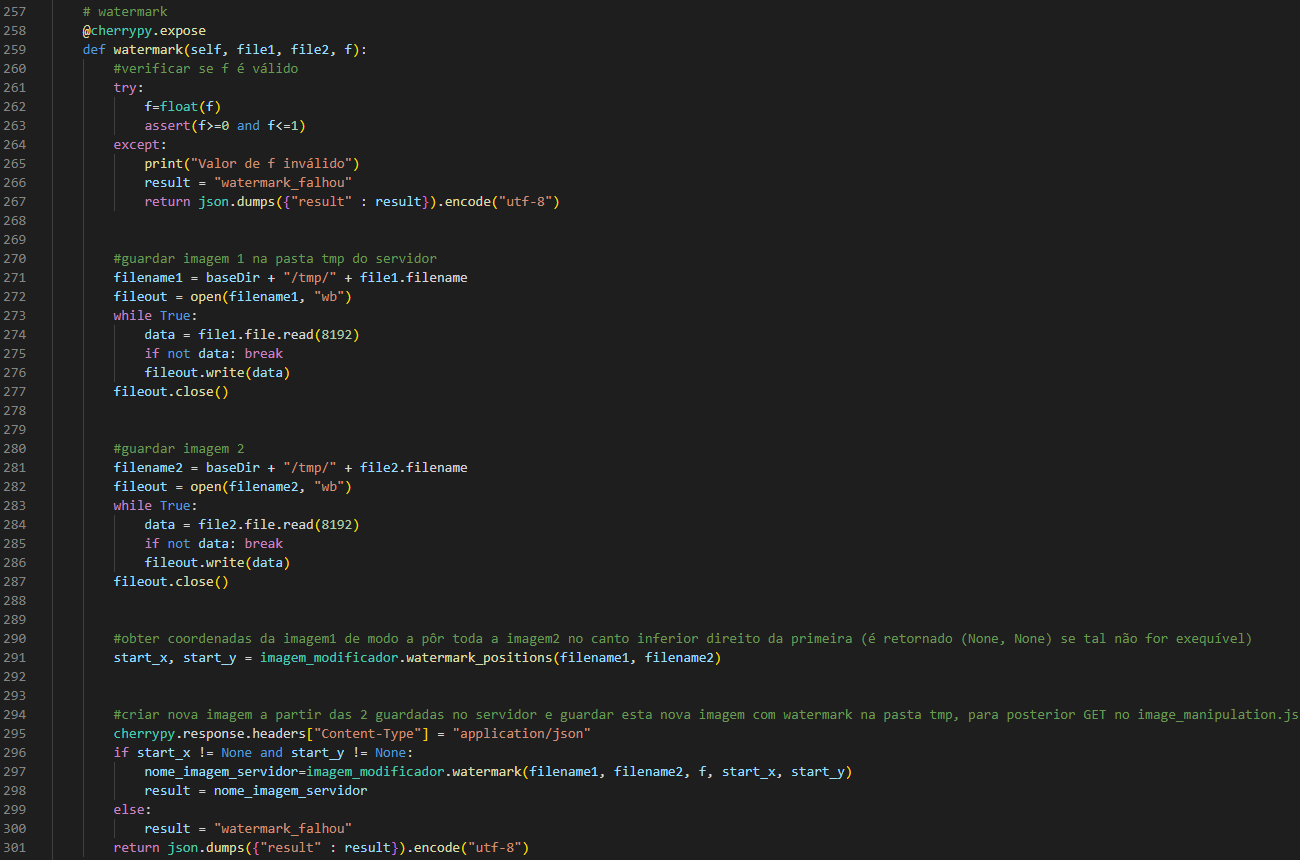
\includegraphics[scale=0.42]{Images_code/12 - image manipulation app watermark.png}
        \caption{\label{Estrutura}Método "watermark".}
\end{figure}


\newpage
\begin{figure}[!hbtp]
        \centering
        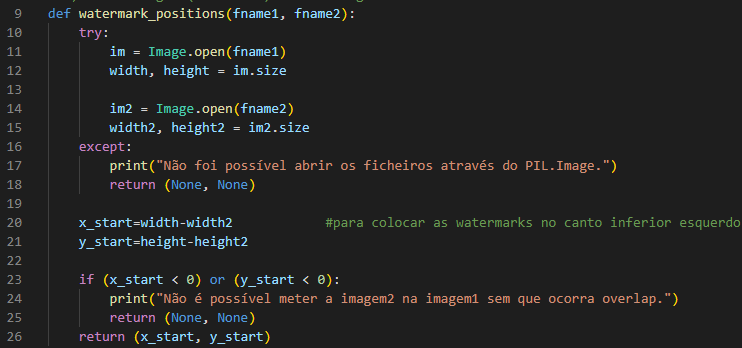
\includegraphics[scale=0.57]{Images_code/12 - image manipulation app2 watermark positions.png}
        \caption{\label{Estrutura}Método "watermark\_positions" do módulo "imagem\_modificador", importado do ficheiro auxiliar mencionado.}
\end{figure}

\begin{figure}[!hbtp]
        \centering
        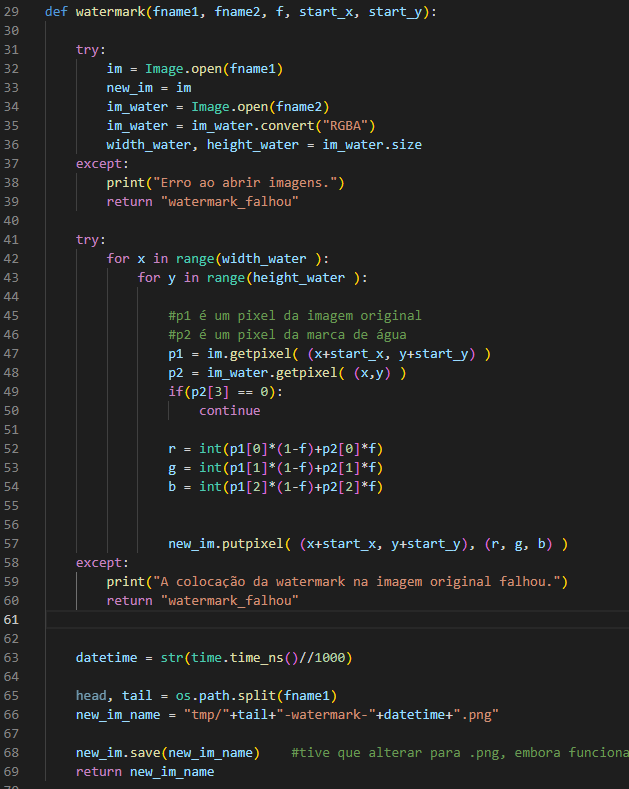
\includegraphics[scale=0.5]{Images_code/12 - image manipulation app2 watermark.png}
        \caption{\label{Estrutura}Método "watermark" do módulo "imagem\_modificador".}
\end{figure}
\newpage



    As funções e métodos explícitos nas últimas 7 páginas, bem como as suas descrições, foram feitas de modo a implementar o método "watermark", e também para descrever a linha de pensamento seguida, bem como o fluxo de interações entre interface e servidor.
\linebreak
 \bigskip
 Como as descrições do funcionamento das interações entre funções javascript e métodos python e de como imaginámos e pensámos e implementámos as funcionalidades de processamento de imagem são semelhantes entre a manipulação de imagem "watermark" e as restantes, passaremos agora para uma exposição de código mais intensa.

\linebreak
 \bigskip
 Segue-se agora a exposição do código do método de manipulação de imagem "bordador", com o código da função "im\_bordador\_inputs", responsável por adicionar à página html os inputs necessários para que o servidor possa manipular a imagem conforme os desejos do utilizador.


\begin{figure}[!hbtp]
        \centering
        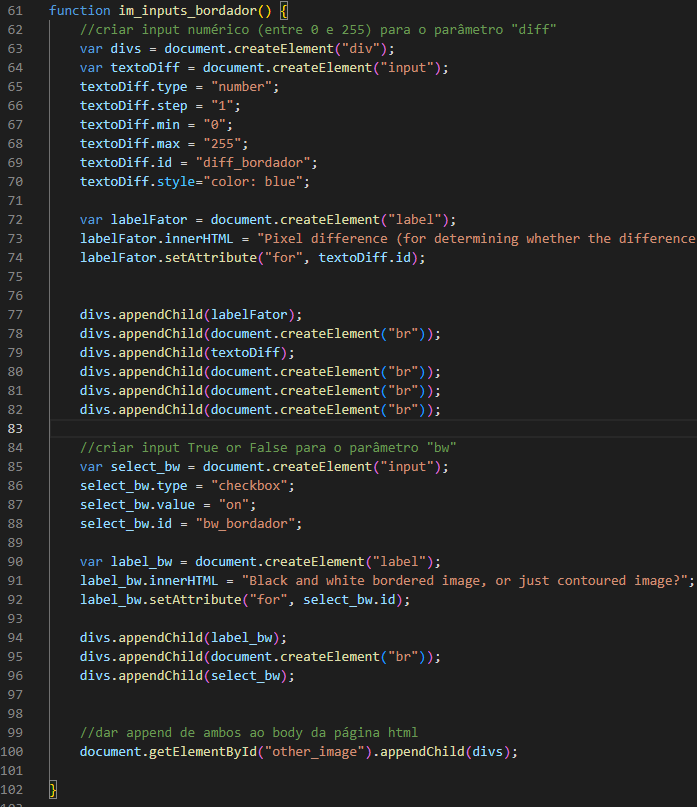
\includegraphics[scale=0.5]{Images_code/13 - image manipulation js bordador im_inputs_bordador.png}
        \caption{\label{Estrutura}Função "im\_bordador\_inputs".}
\end{figure}

\newpage
\begin{figure}[!hbtp]
        \centering
        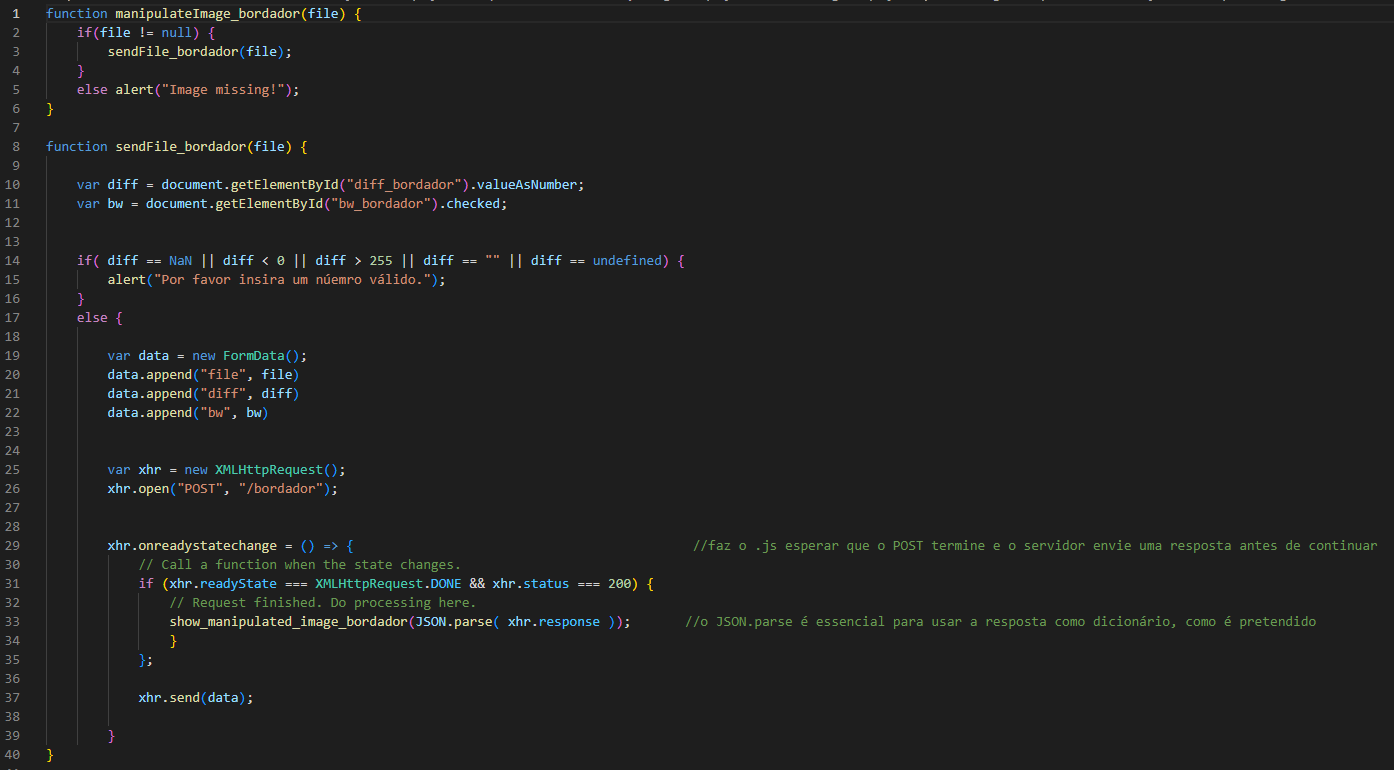
\includegraphics[scale=0.4]{Images_code/13 - image manipulation js bordador manipulateImage_bordador e sendfile_bordador.png}
        \caption{\label{Estrutura}Função "manipulateImage\_bordador", invocada quando se clica no botão de submeter aquando este método "bordador" está selecionado, e função "sendfile\_bordador", que envia o POST ao servidor.}
\end{figure}

\begin{figure}[!hbtp]
        \centering
        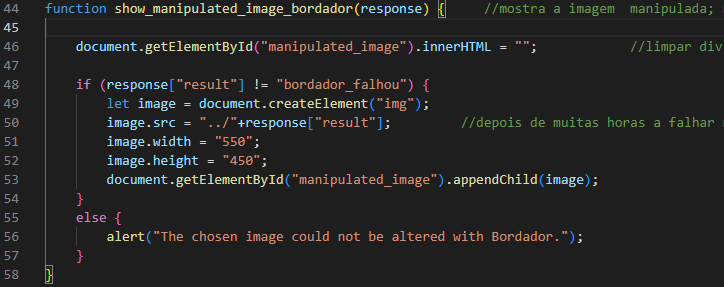
\includegraphics[scale=0.8]{Images_code/13 - image manipulation js bordador show_manipulated_image_bordador.png}
        \caption{\label{Estrutura}Função "show\_manipulates\_image\_bordador", responsável por interpretar o objeto json recebido do servidor e mostrar a imagem resultante, ou uma mensagem de erro, conforme o conteúdo do mesmo.}
\end{figure}

\newpage

    Do lado do servidor, relativamente à funcionalidade de manipulação de imagem "bordador":

    \begin{figure}[!hbtp]
        \centering
        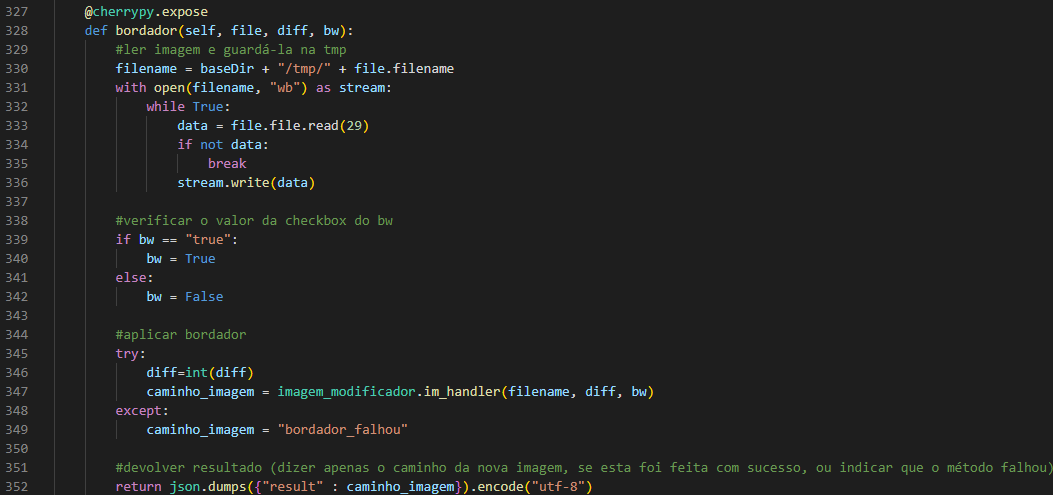
\includegraphics[scale=0.54]{Images_code/13 - image manipulation app bordador.png}
        \caption{\label{Estrutura}Método "bordador".}
\end{figure}

\linebreak
 \bigskip
 \bigskip
 \bigskip
 
    E o devido método proveniente do módulo "image\_modificador" mostrado na imagem acima, que é complexo (constituído por 3 métodos distintos), que marca as bordas na imagem recebida (enviada pela interface através do POST, com o parâmetro de diferença entre píxeis a considerar até a considerar como borda, bem como o parâmetro booleano de obter uma imagem em black and white, com as bordas a serem delimitadas numa cor, e os restantes píxeis noutra cor, ou de obter uma imagem em que apenas as bordas são delimitadas, retendo os restantes píxeis as suas qualidades já existentes).


\newpage

    \begin{figure}[!hbtp]
        \centering
        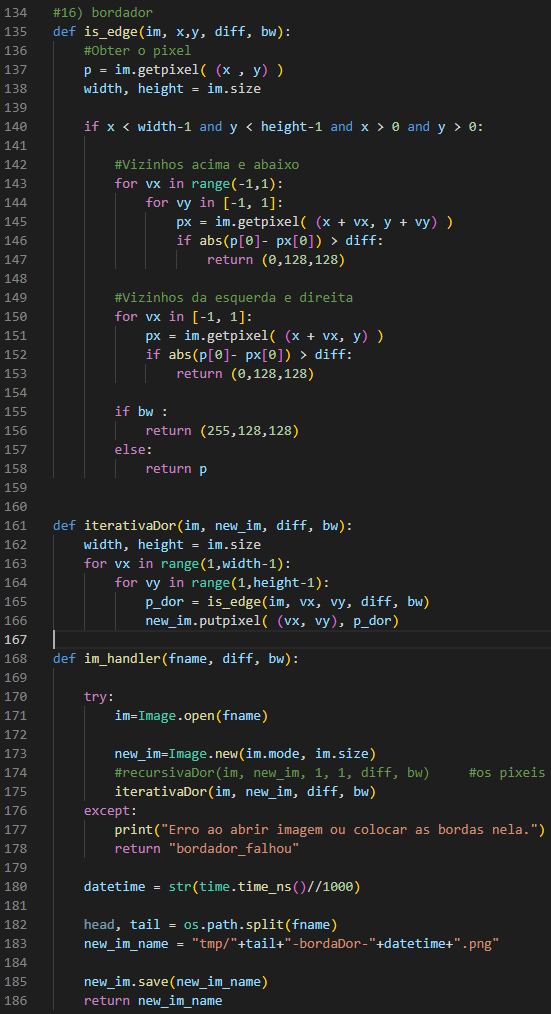
\includegraphics[scale=0.62]{Images_code/13 - image manipulation app2 bordador.png}
        \caption{\label{Estrutura}Métodos auxiliares do módulo "image\_modificador" para ajudar o método "bordador" no servidor a servir a imagem pretendida, modificada segundo os parâmetros pretendidos.}
\end{figure}



\newpage

    Vistas as implementações destes 2 métodos de manipulação de imagem ("watermark" e "bordador"), não mostraremos as implementações das restantes 7 (ou mais corretamente, 13 métodos restantes, tendo em conta as derivações que os métodos "sepsis/lomography", "resizer", e "unknown" contém).
    

\linebreak
 \bigskip

 Mostraremos agora, para terminar este capítulo, uma função e método de nome idêntico que são chamados quando a página de Image Manupulation é fechada, e que têm como objetivo limpar a pasta ./tmp.

\linebreak
 \bigskip
 

\begin{figure}[!hbtp]
        \centering
        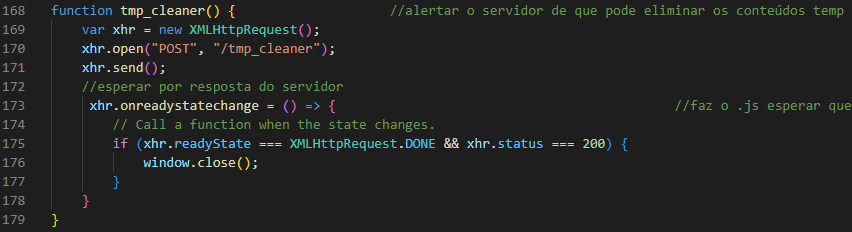
\includegraphics[scale=0.6]{Images_code/12 - image manipulation js tmp_cleaner.png}
        \caption{\label{Estrutura}Função "tmp\_cleaner", chamada quando a página Image Manipulation é fechada.}
\end{figure}

\linebreak
 \bigskip

\begin{figure}[!hbtp]
        \centering
        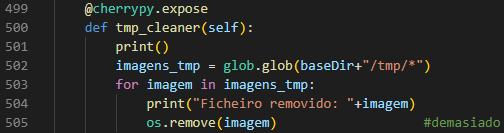
\includegraphics[scale=0.9]{Images_code/12 - image manipulation app tmp_cleaner.png}
        \caption{\label{Estrutura}Método "tmp\_cleaner", chamado pelo POST enviado pela função de nome verossimilhante.}
\end{figure}

\newpage






















 


\chapter{Resultados}
\label{chap.resultados}

A aplicação WEB que nos foi proposta visa gerir imagens; carregá-las, guardá-las, visualizá-las e manipulá-las. A aplicação WEB que desenvolvemos seguindo a metodologia descrita, permite o uso de todas essas funcionalidades.

\linebreak
 \bigskip
 
 Nós testámos e usufruímos da nossa aplicação WEB através da interface da aplicação, que pode ser usada a partir dum browser comum, inserindo o endereço ‘127.0.0.1:10013’ no mesmo. 

\linebreak
 \bigskip
 
    Como já referido, decidimos implementar um mecanismo de registo/login antes de permitirmos o acesso de alguém às funcionalidades descritas. A imagem abaixo mostra o que se pode ver após a inserção do endereço mencionado acima no navegador:

    \begin{figure}[!hbtp]
        \centering 
        
\includegraphics[scale=0.260]{Images/pagina_login.png}
        \caption{\label{Login}Página de LogIn/Registo}
    \end{figure}

    \newpage
    
    Um utilizador pode criar uma conta (caso não tenha) ao preencher os campos “Username” e “Password” como pretender e clicar em “Register”, sendo que o nome de utilizador tem de ser único (é mostrado um alerta caso o utilizador se tente registar com um nome de utilizador já existente na base de dados).

    \bigskip

    \begin{figure}[!hbtp]
        \centering 
        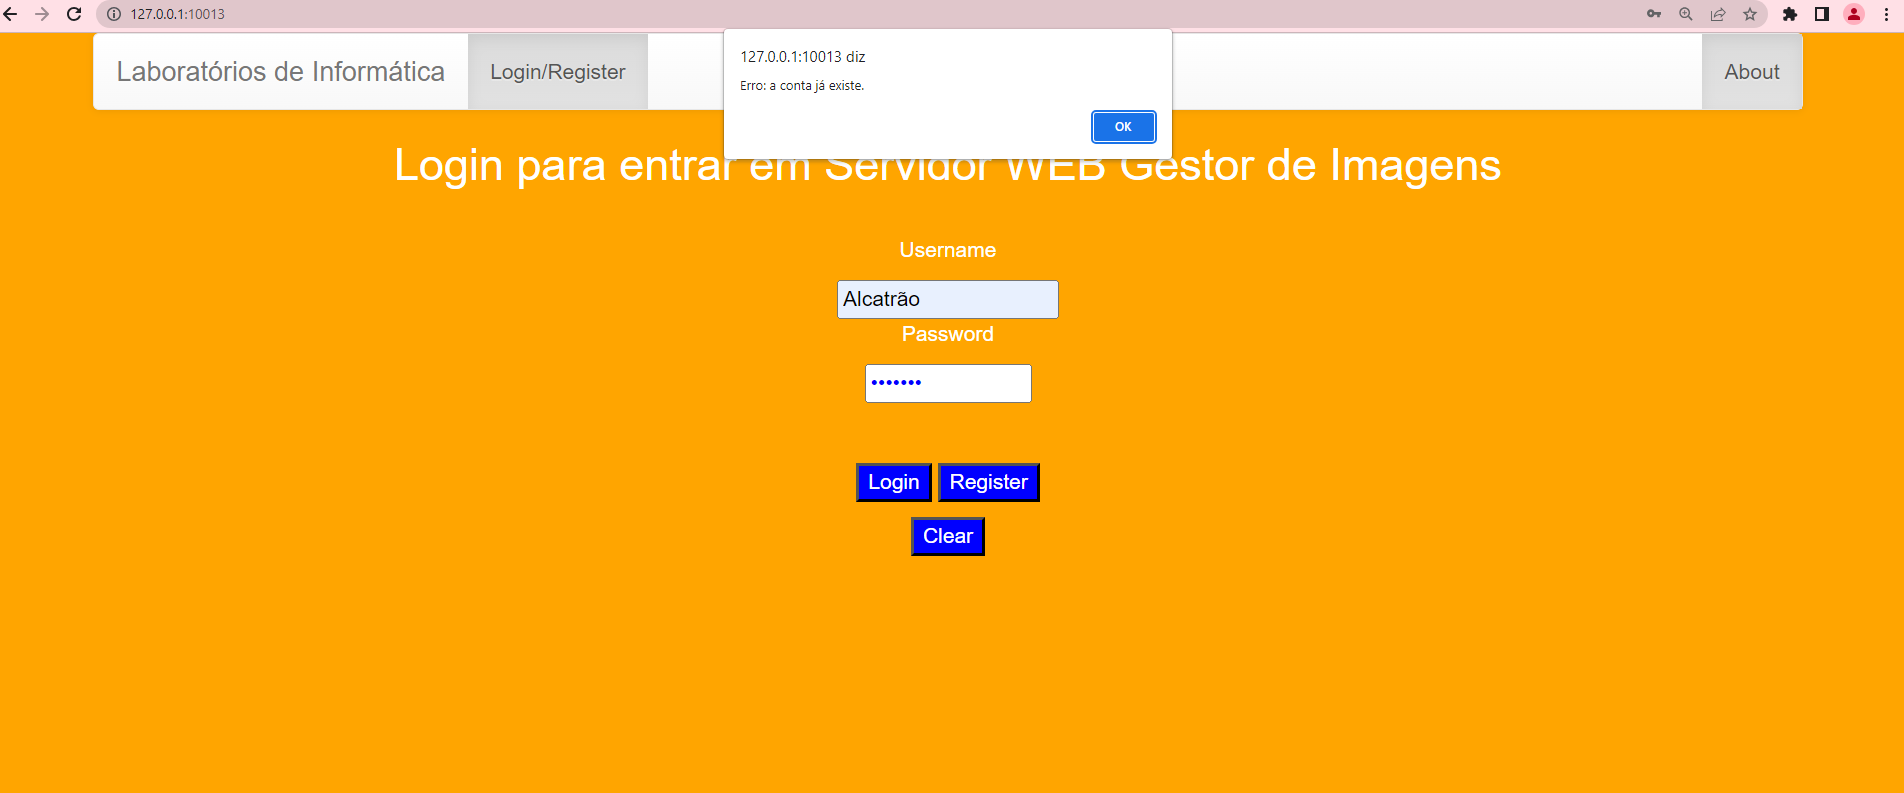
\includegraphics[scale=0.260]{Images/pagina_inicial_registo_failed.png}
        \caption{\label{Erro}Erro de Registo de Utilizador}
    \end{figure}

    Caso as credenciais inseridas sejam validadas com sucesso pelo servidor WEB, é mostrada ao invés uma mensagem a indicar esse sucesso.

    \linebreak
    \bigskip
    \bigskip
 
    Tendo a conta criada, o utilizador pode proceder para a página principal ao clicar em “Login” com as credenciais com que criou a conta.

    \begin{figure}[!hbtp]
        \centering 
        \includegraphics[scale=0.260]{Images/página principal.png}
        \caption{\label{Home}Página Principal após login}
    \end{figure}

\newpage


    Nesta nova página, o utilizador pode observar na barra de navegação opções que não conseguia ver antes: a Gallery Page, a UpLoad Page, e a Image Manipulation Page. As funcionalidades destas páginas já foram descritas na Introdução (Estrutura; organização visual) e também foram descritas extensivamente ao longo da Metodologia. Ao clicar numa destas opções, será apresentada ao utilizador, numa nova janela, uma página que permita ao mesmo fazer uso de funcionalidades que podem ser inferidas pelo nome da página.

         \linebreak
    \bigskip
    Sem mais detalhes, visualizemos os resultados que se podem observar em cada página.

    \begin{figure}[!hbtp]
        \centering 
        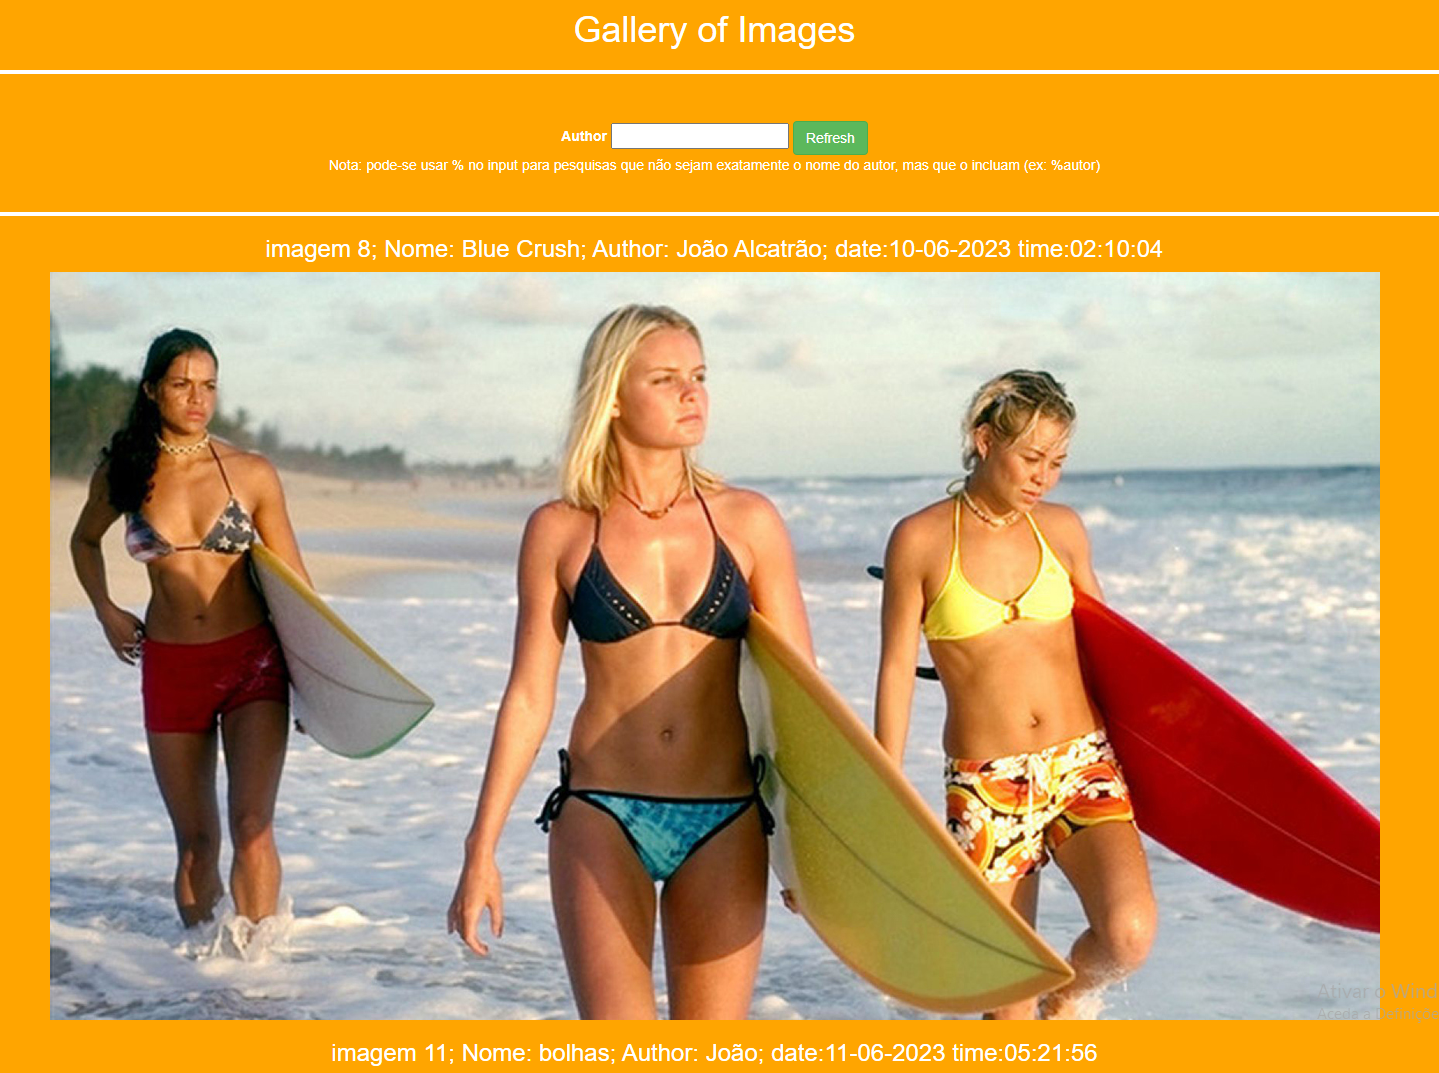
\includegraphics[scale=0.350]{Images_code/0 - galeria.png}
        \caption{\label{Gallery}Gallery Page.}
    \end{figure}

    \begin{figure}[!hbtp]
        \centering 
        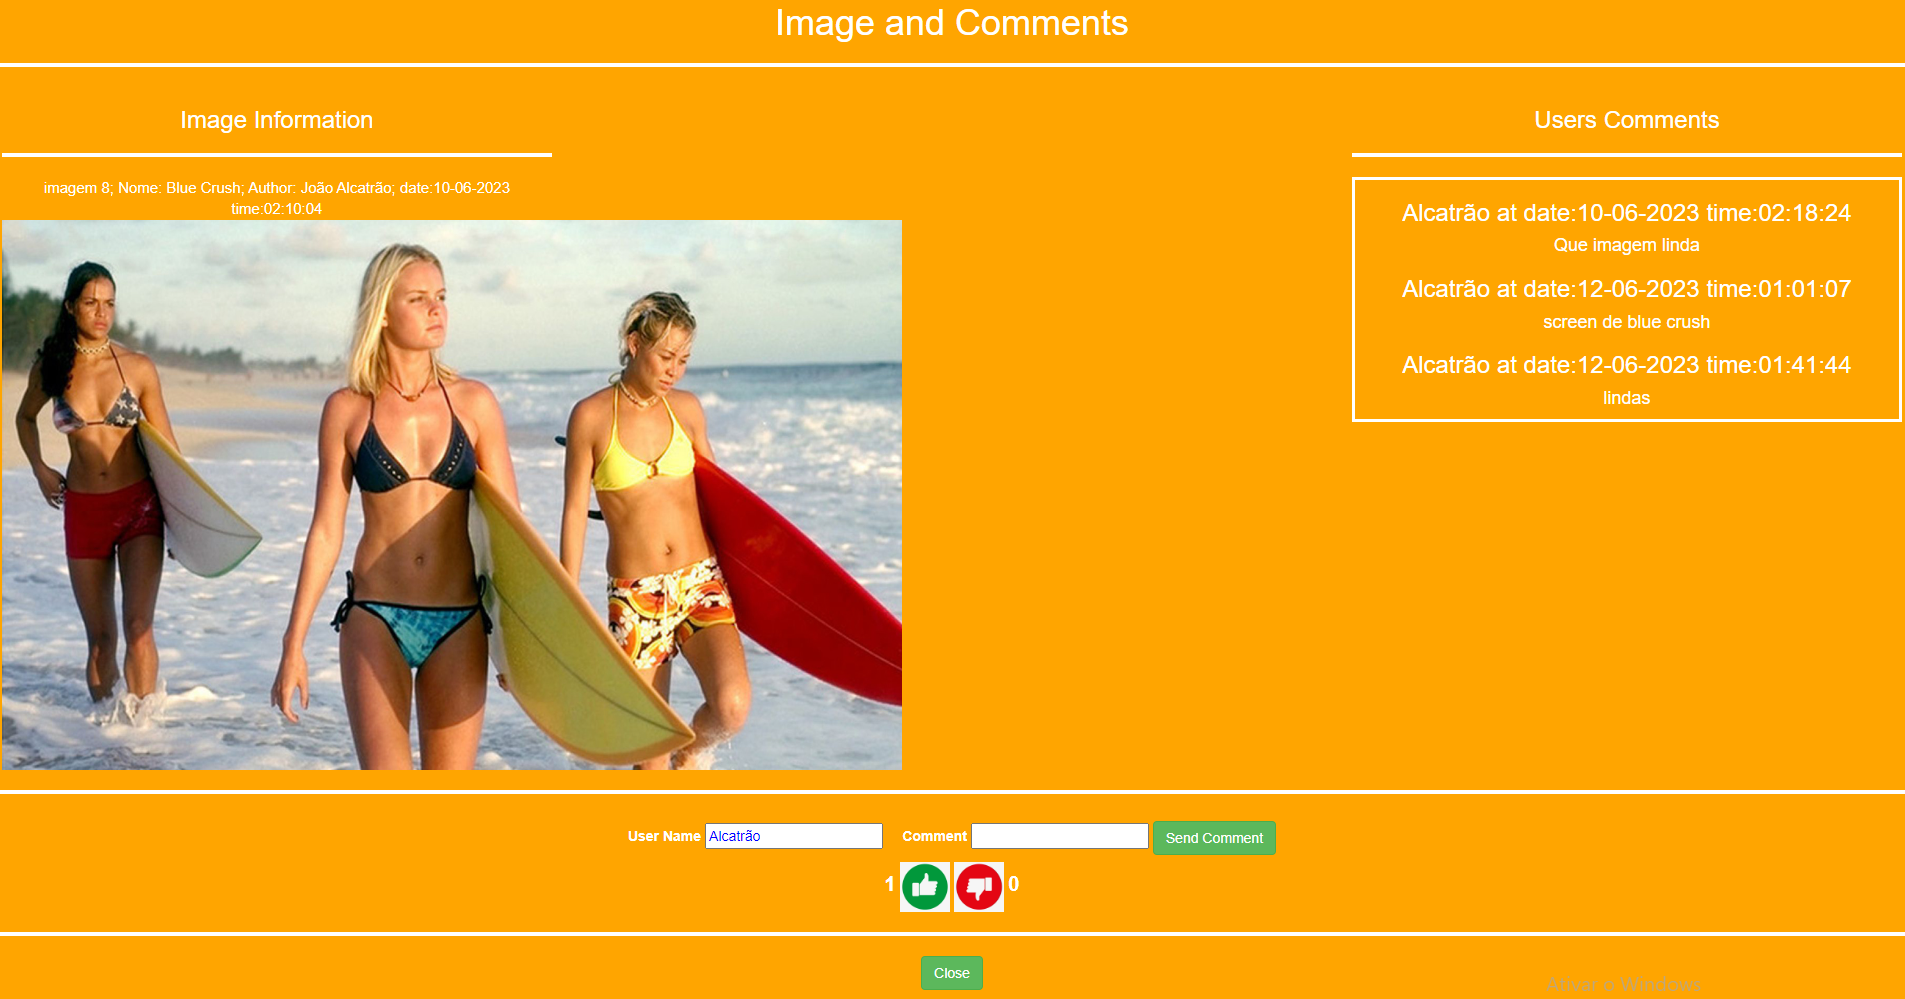
\includegraphics[scale=0.29]{Images_code/0 - imagem, comments, gostos.png}
        \caption{\label{Image}Image Page.}
    \end{figure}


    \begin{figure}[!hbtp]
        \centering 
        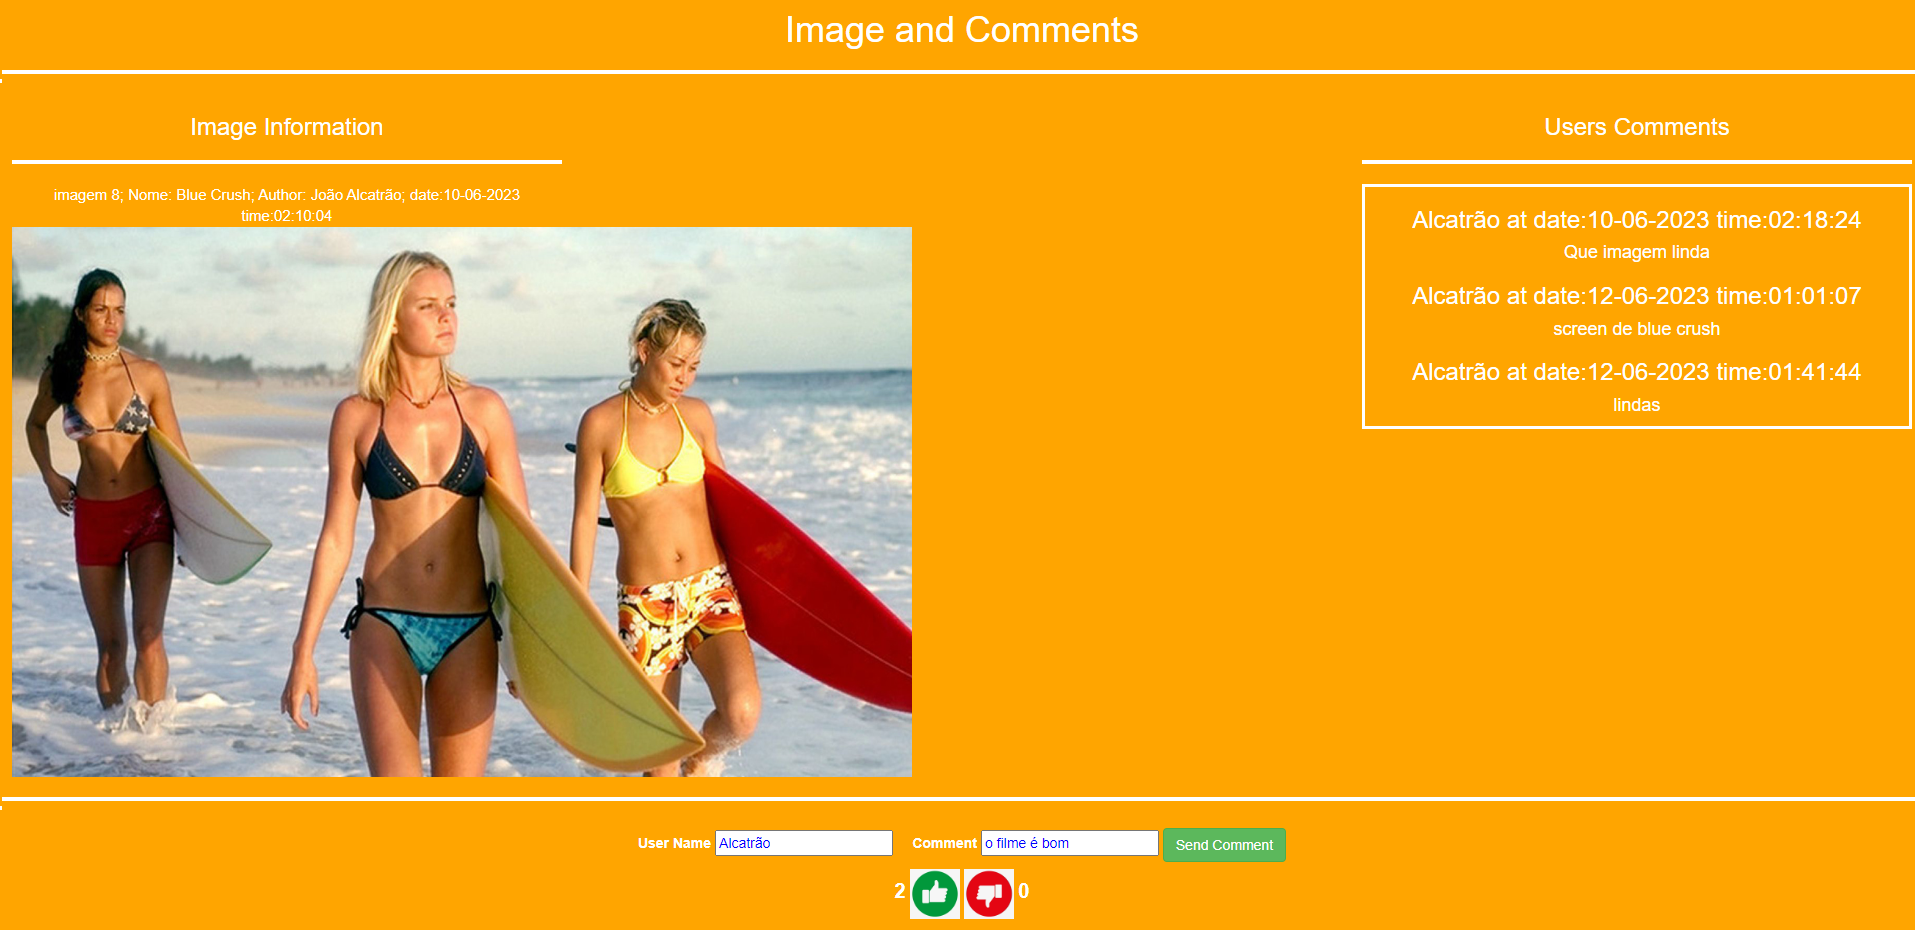
\includegraphics[scale=0.29]{Images_code/0 - imagem, comments, gostos 2.png}
        \caption{\label{Image}Image Page (escrevendo um comentário após fazer um gosto à imagem).}
    \end{figure}

    \begin{figure}[!hbtp]
        \centering 
        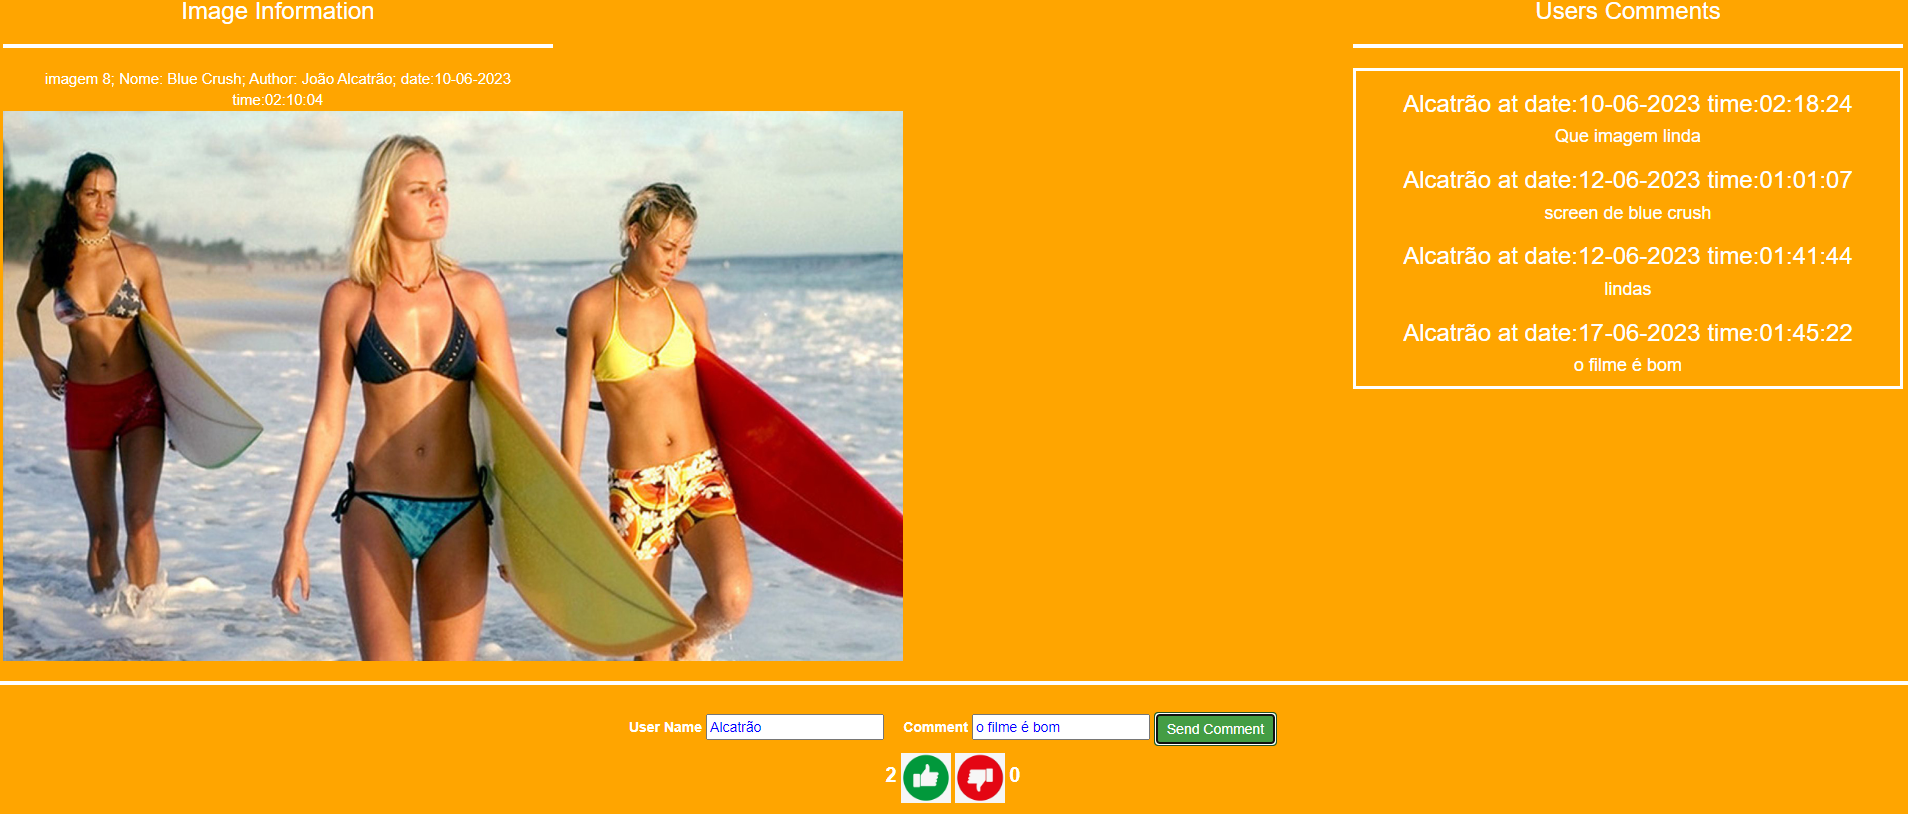
\includegraphics[scale=0.29]{Images_code/0 - imagem, comments, gostos 3.png}
        \caption{\label{Image}Image Page (após submeter o comentário).}
    \end{figure}

    \begin{figure}[!hbtp]
        \centering 
        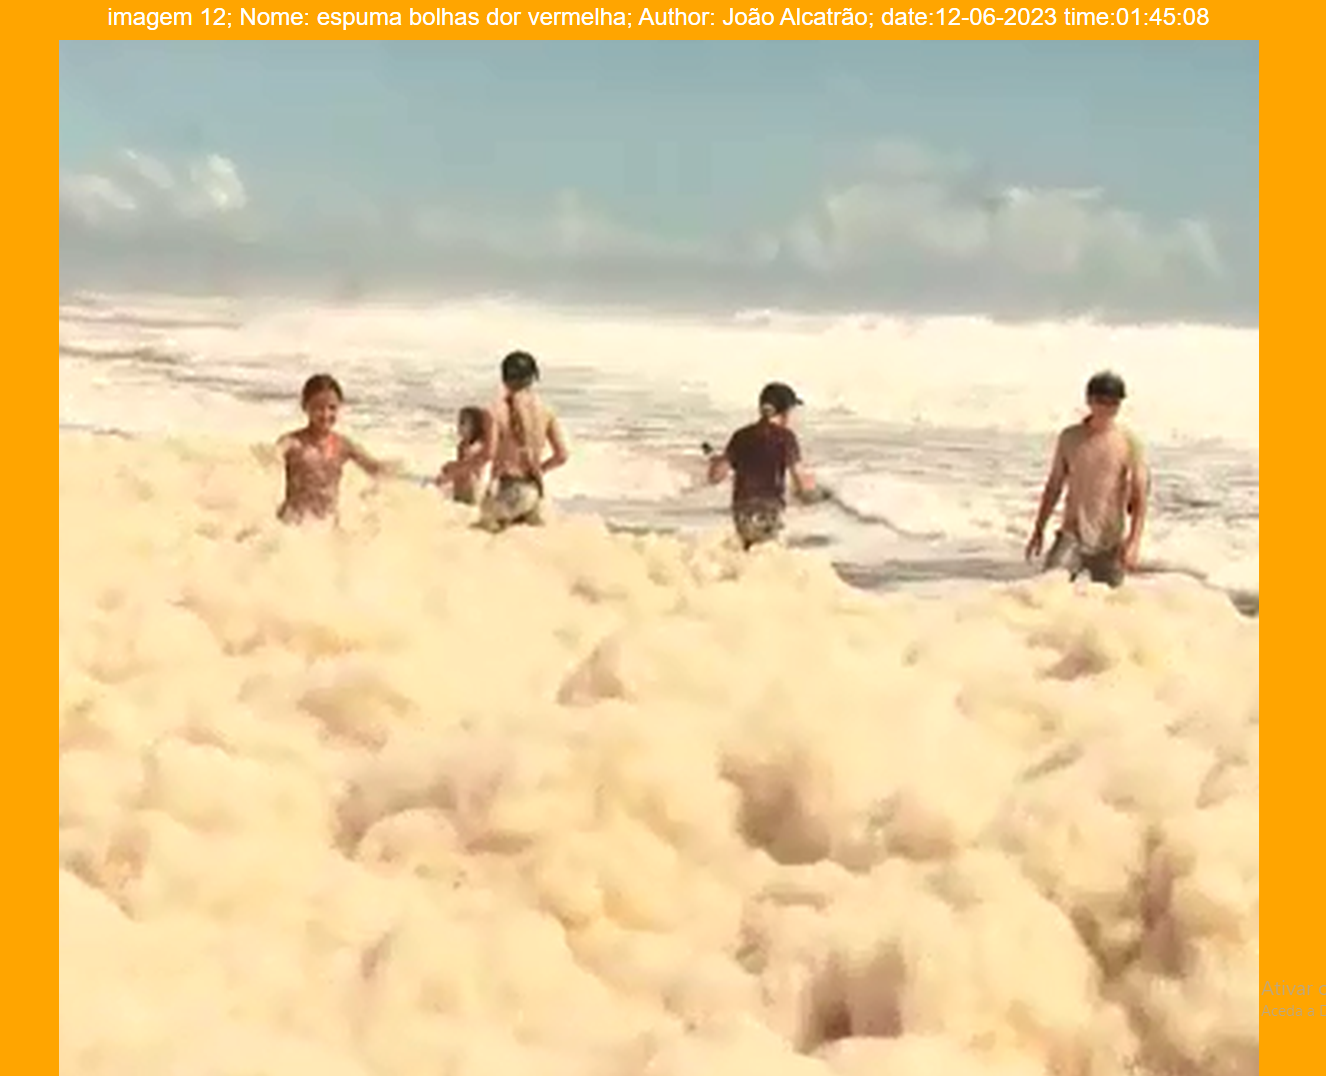
\includegraphics[scale=0.450]{Images_code/0 - galeria 2.png}
        \caption{\label{Upload}Gallery Page (scroll mais para o fundo da página).}
    \end{figure}

    \begin{figure}[!hbtp]
        \centering 
        
\includegraphics[scale=0.290]{Images_code/0 - upload.png}
        \caption{\label{Upload}Upload Page.}
    \end{figure}

    \begin{figure}[!hbtp]
        \centering 
        \includegraphics[scale=0.29]{Images_code/0 - upload 2.png}
        \caption{\label{Upload}Upload Page (visualização de uma imagem escolhida, e do nome que lhe se quer dar).}
    \end{figure}

      \begin{figure}[!hbtp]
        \centering 
        \includegraphics[scale=0.29]{Images_code/0 - image manipulation.png}
        \caption{\label{Image Manipulation}Image Manipulation Page.}
    \end{figure}

    \begin{figure}[!hbtp]
        \centering 
        \includegraphics[scale=0.29]{Images_code/0 - image manipulation 2.png}
        \caption{\label{Image Manipulation}Image Manipulation Page (escolher uma imagem).}
    \end{figure}

    \begin{figure}[!hbtp]
        \centering 
        \includegraphics[scale=0.29]{Images_code/0 - image manipulation 3.png}
        \caption{\label{Image Manipulation}Image Manipulation Page (escolher um método).}
    \end{figure}

    \begin{figure}[!hbtp]
        \centering 
        \includegraphics[scale=0.29]{Images_code/0 - image manipulation 4.png}
        \caption{\label{Image Manipulation}Image Manipulation Page (escolher outra imagem e meter um valor decimal no campo mostrado, como é pedido pelo método escolhido).}
    \end{figure}

    \begin{figure}[!hbtp]
        \centering 
        \includegraphics[scale=0.29]{Images_code/0 - image manipulation 5.png}
        \caption{\label{Image Manipulation}Image Manipulation Page (resultado da submissão das imagens escolhidas e do fator de transparência escolhido).}
    \end{figure}

    \begin{figure}[!hbtp]
        \centering 
        \includegraphics[scale=0.29]{Images_code/0 - image manipulation 6_0.png}
        \caption{\label{Image Manipulation}Image Manipulation Page (selecionar outra imagem secundária).}
    \end{figure}

    \begin{figure}[!hbtp]
        \centering 
        \includegraphics[scale=0.29]{Images_code/0 - image manipulation 6.png}
        \caption{\label{Image Manipulation}Image Manipulation Page (resultado da submissão com os novos parâmetros).}
    \end{figure}

    \begin{figure}[!hbtp]
        \centering 
        \includegraphics[scale=0.29]{Images_code/0 - image manipulation 7.png}
        \caption{\label{Image Manipulation}Image Manipulation Page (escolha de outra imagem e método de manipulação, e resultado da sua submissão ao servidor).}
    \end{figure}

    \begin{figure}[!hbtp]
        \centering 
        \includegraphics[scale=0.29]{Images_code/0 - image manipulation 8.png}
        \caption{\label{Image Manipulation}Image Manipulation Page (escolha de outra imagem e método de manipulação e da opção desejada, e resultado da sua submissão).}
    \end{figure}

    \begin{figure}[!hbtp]
        \centering 
        \includegraphics[scale=0.29]{Images_code/0 - image manipulation 9.png}
        \caption{\label{Image Manipulation}Image Manipulation Page (escolha de outra imagem e método de manipulação e de um valor no campo mostrado, e resultado da sua submissão).}
    \end{figure}

    \begin{figure}[!hbtp]
        \centering 
        \includegraphics[scale=0.29]{Images_code/0 - image manipulation 10.png}
        \caption{\label{Image Manipulation}Image Manipulation Page (escolha de outra imagem e método de manipulação e do valor de saturação desejado, e resultado da sua submissão).}
    \end{figure}




    

    

\chapter{Análise}
\label{chap.analise}
Analisando os resultados obtidos, das quais as images acima mostram o essencial do que a nossa aplicação consegue fazer, mas não tudo, podemos afirmar que conseguimos cumprir os objetivos que nos foram propostos, e conseguimo-lo usando boas práticas.

\linebreak
\bigskip

Estudando cada funcionalidade que a aplicação tinha de ter e que implementámos:

\linebreak
\bigskip
\bigskip

    \textbf{Login/register:} a nossa aplicação tem um sistema de registo/login, que permite que apenas os utilizadores que criem conta na nossa aplicação possa usufruir totalmente dela (há livre acesso à página About e à própria página de registo/login apenas). Isto não serve apenas para frustrar os utilizadores, antes pelo contrário: permite que cada utilizador seja unicamente identificado pelo seu nome, e que mais nenhum outra possa fazer ações na aplicação sob o seu nome. O utilizador, ao criar conta e fazer login, verá que os campos de autor da página de carregamento de imagens e da página de apreciação e comentário de cada imagem já estarão preenchidos com o seu nome quando entrar nestas páginas. 
    
    \linebreak
    \bigskip
    
    O sistema pode parecer pouco ortodoxo, considerando que usamos um userID fabricado a partir da junção do nome de utilizador com a síntese da junção do nome de utilizador com a síntese da password para controlar o acesso dos utilizadores às diversas páginas da nossa aplicação. De qualquer modo, os objetivos de garantir a unicidade do utilizador na aplicação, e de garantir que a página de login/registo não possa ser facilmente ultrapassada adicionando uma expressão genérica e previsível no endereço, como "/html/upload", encontram-se cumpridos.
    
    \newpage
    
    \textbf{Carregamento de imagens:} a nossa aplicação permite ao utilizador carregar imagens ao seu agrado na página Upload, separando a visualização do carregamento da mesma (o que permite ao utilizador alterar a sua escolha de imagem sem a carregar no sistema) e permite-o dar o nome que pretender que essas imagens apresentem na galeria do servidor.
    
    \linebreak
    \bigskip
    
    A data e a hora do carregamento da imagem também são registadas pelo servidor na base de dados, e pode-se ver estas observações na galeria, e na página de apreciação (comentários e gostos) da respetiva imagem. Além disso, fomos além e garantimos que ninguém, a não ser o próprio utilizador em questão, possa submeter imagens sob o nome do próprio. A sua identidade é preservada, protegida e mantida.
    
    \linebreak
    \bigskip
    \bigskip
    \bigskip
    
    \textbf{Visualização de imagens:} a nossa aplicação permite ao utilizador usar a página Gallery para ver uma lista de todas as imagens presentes no sistema, ordenadas por ordem ascendente do nome, permitindo a sua visualização. As imagens
em sí estão armazenadas no sistema de ficheiros da aplicação Web (renomeadas de acordo com a sua síntese SHA256 para evitar que imagens essencialmente diferentes mas com nomes idênticos se substituam), mas as informações que as acompanham (nome que o utilizador que a carregou lhe deu, o nome desse autor, e a data e hora e de carregamento) são registadas na base de dados.

\linebreak
\bigskip

    Além disso, é possível filtrar as imagens mostradas pelo autor, sendo possíveis tanto filtragens parciais como absolutas, como é indicado na página. Esta filtragem baseia-se em pesquisas na base de dados, pelo que tivémos o cuidado de usar boas práticas a escrever o nosso código para evitar SQL injection.
    
    \newpage
    
    \textbf{Apreciação de imagem:} quando uma imagem é selecionada na galeria, é aberta uma nova página autónoma que apresenta todas as suas propriedades (autor, nome, hora e data de upload no sistema, comentários efetuados pelos utilizadores, e os gostos/desgostos deixados pelos mesmos). Esta página permite ao utilizador fazer os seus próprios comentários de forma exclusiva, com a garantia de que mais ninguém pode comentar sob o seu nome (tal como ocorre no carregamento de imagens).
    
    \linebreak
    \bigskip
    
    Por último, é permitido ao utilizador facilmente fazer gostos/desgostos com um simples clique, e permite também retirá-los de igual forma com um clique (clicar duas vezes seguidas no botão gosto, adiciona na primeira instância um gosto à imagem, e retira na segunda esse gosto à imagem, tal como é o comportamento observado em funcionalidades semelhantes de algumas aplicações mais populares, como o Facebook e o Instagram. Isto é feito ao inserir e remover registos na base de dados, em especial os registos pertencentes ao utilizador que fez/desfez esses gostos/desgostos, garantindo assim consistência na aplicação, e garantindo que um utilizador que faça um gosto, feche e volte a abrir a página, e que volte a fazer gosto, acaba por desfazer o gosto que tinha inicialmente feito).
    
    \linebreak
    \bigskip
    \bigskip
    \bigskip
    
    \textbf{Manipulação de imagens:} a nossa aplicação contém, na página de manipulação de imagens, uma vasta gama de métodos de processamento de imagens, bem como opções dentro de cada método que permitem ao utilizador manipular imagens como realmente desejar e pretender. Para facilitar a comparação entre a imagem original e a manipulada, a página mostra ambas lado a lado, e permite ao utilizador guardar a imagem manipulada no seu computador (de onde ele também pode carregar a imagem que deseja manipular).
    
    \linebreak
    \bigskip
    
    Os diversos métodos de manipulação de imagem têm um conjunto de verificações aos parâmetros escolhidos que são feitas tanto do lado da interface, em javascript, como no lado do servidor, em python. As verificações do lado da interface servem mais para facilitar o processo de manipulação de imagem ao utilizador, enquanto que as verificações do lado do servidor servem para assegurar o bom funcionamento e segurança do sistema o quão melhor que consiga.

    \newpage
    Para terminar esta secção, apresentamos agora alguns dos testes unitários e funcionais que fizémos para assegurar o bom funcionamento do sistema, e garantir que este continue a correr em segurança, mesmo no caso de receber parâmetros e dados questionáveis. Fizémos um total de 43 testes, alguns com parâmetros válidos, a maioria com parâmetros inválidos, e garantimos que os nossos métodos passam neles todos.

    \begin{figure}[!hbtp]
        \centering 
        \includegraphics[scale=0.3]{Images_code/15 - testes.png}
        \caption{\label{Testes} Testes unitários aos métodos de manipulação de imagens.}
    \end{figure}

    \begin{figure}[!hbtp]
        \centering 
        \includegraphics[scale=0.9]{Images_code/15 - testes 2.png}
        \caption{\label{Testes} Continuação de testes unitários aos métodos de manipulação de imagens. }
    \end{figure}

    \begin{figure}[!hbtp]
        \centering 
        \includegraphics[scale=0.4]{Images_code/15 - testes 4.png}
        \caption{\label{Testes}Testes de persistência.}
    \end{figure}

    \begin{figure}[!hbtp]
        \centering 
        \includegraphics[scale=1]{Images_code/15 - testes 5.png}
        \caption{\label{Testes}Teste funcional à aplicação com uso de requests.}
    \end{figure}

    \begin{figure}[!hbtp]
        \centering 
        \includegraphics[scale=0.7]{Images_code/15 - testes 6.png}
        \caption{\label{Testes}Teste funcional à aplicação com registo, login, e acesso à página da galeria.}
    \end{figure}

    \begin{figure}[!hbtp]
        \centering 
        \includegraphics[scale=0.7]{Images_code/15 - testes 6.png}
        \caption{\label{Testes}Teste simples aos métodos de acesso a páginas do servidor.}
    \end{figure}

    \begin{figure}[!hbtp]
        \centering 
        \includegraphics[scale=0.54]{Images_code/16 - teste resultado.png}
        \caption{\label{Testes}Resultado da execução dos testes.}
    \end{figure}
    
    

\chapter{Conclusões}
\label{chap.conclusao}
Todos os objetivos forma cumpridos, todas as funcionalidades foram implementadas, e estamos imensamente satisfeitos com os resultados da nossa aplicação. Tendo em conta tudo o que foi demonstrado ao longo deste relatório, podemos afirmar que a nossa solução é complexa e foi muito trabalhada. Aprofundámos agudamente os nossos conhecimentos em Javascript e Cherrypy, através de programação exaustiva nesta linguagem e framework, e solidificámos as nossas competência em programação Python, em SQL, tivémos novas experiências com HTML e CSS e LaTeX, e aplicámos métodos aprendidos ao longo da disciplina relativos a criptografia e testagem. 

\linebreak
\bigskip

Desejamos terminar este relatório afirmando que estamos satisfeitos com o trabalho que fizémos, com a perserverância que demonstrámos para com nós próprios, e sentimos-nos felizes com a aplicação criada, a nossa bela aplicação.

\chapter*{Contribuições dos autores}
João Alcatrão - interface (html, css, javascript), servidor e métodos de manipulação de imagem (cherrypy, python), base de dados (sql), testes unitários e funcionais, relatório

\linebreak
\bigskip

José Jordão - interface (html, css), servidor e métodos de manipulação (cherrypy, python), relatório (latex)

\linebreak
\bigskip

Mónica Pereira - servidor (cherrypy, python), base de dados (sql), relatório
\linebreak

Pedro Costa - relatório (latex)


\vspace{10pt}


\autores : 
\\

\quad\qquad 25\%  \qquad\quad\quad  25\%   \quad\quad\quad\quad   25\%   \quad\quad\quad\quad    25\%\\

%%%%%%%%%%%%%%%%%%%%%%%%%%%%%%%%%
\chapter*{GitHub e XCOA}

GitHub: 

\linebreak

\href{https://github.com/detiuaveiro/projeto-final-labi2023g13}{https://github.com/detiuaveiro/projeto-final-labi2023g13}

\linebreak
\bigskip
\bigskip
\bigskip

XCOA: 

\linebreak
\href{https://xcoa.av.it.pt/labiproj13}{https://xcoa.av.it.pt/labiproj13}


%%%%%%%%%%%%%%%%%%%%%%%%%%%%%%%%%
\printbibliography

\end{document}